\documentclass[1p]{elsarticle_modified}
%\bibliographystyle{elsarticle-num}

%\usepackage[colorlinks]{hyperref}
%\usepackage{abbrmath_seonhwa} %\Abb, \Ascr, \Acal ,\Abf, \Afrak
\usepackage{amsfonts}
\usepackage{amssymb}
\usepackage{amsmath}
\usepackage{amsthm}
\usepackage{scalefnt}
\usepackage{amsbsy}
\usepackage{kotex}
\usepackage{caption}
\usepackage{subfig}
\usepackage{color}
\usepackage{graphicx}
\usepackage{xcolor} %% white, black, red, green, blue, cyan, magenta, yellow
\usepackage{float}
\usepackage{setspace}
\usepackage{hyperref}

\usepackage{tikz}
\usetikzlibrary{arrows}

\usepackage{multirow}
\usepackage{array} % fixed length table
\usepackage{hhline}

%%%%%%%%%%%%%%%%%%%%%
\makeatletter
\renewcommand*\env@matrix[1][\arraystretch]{%
	\edef\arraystretch{#1}%
	\hskip -\arraycolsep
	\let\@ifnextchar\new@ifnextchar
	\array{*\c@MaxMatrixCols c}}
\makeatother %https://tex.stackexchange.com/questions/14071/how-can-i-increase-the-line-spacing-in-a-matrix
%%%%%%%%%%%%%%%

\usepackage[normalem]{ulem}

\newcommand{\msout}[1]{\ifmmode\text{\sout{\ensuremath{#1}}}\else\sout{#1}\fi}
%SOURCE: \msout is \stkout macro in https://tex.stackexchange.com/questions/20609/strikeout-in-math-mode

\newcommand{\cancel}[1]{
	\ifmmode
	{\color{red}\msout{#1}}
	\else
	{\color{red}\sout{#1}}
	\fi
}

\newcommand{\add}[1]{
	{\color{blue}\uwave{#1}}
}

\newcommand{\replace}[2]{
	\ifmmode
	{\color{red}\msout{#1}}{\color{blue}\uwave{#2}}
	\else
	{\color{red}\sout{#1}}{\color{blue}\uwave{#2}}
	\fi
}

\newcommand{\Sol}{\mathcal{S}} %segment
\newcommand{\D}{D} %diagram
\newcommand{\A}{\mathcal{A}} %arc


%%%%%%%%%%%%%%%%%%%%%%%%%%%%%5 test

\def\sl{\operatorname{\textup{SL}}(2,\Cbb)}
\def\psl{\operatorname{\textup{PSL}}(2,\Cbb)}
\def\quan{\mkern 1mu \triangleright \mkern 1mu}

\theoremstyle{definition}
\newtheorem{thm}{Theorem}[section]
\newtheorem{prop}[thm]{Proposition}
\newtheorem{lem}[thm]{Lemma}
\newtheorem{ques}[thm]{Question}
\newtheorem{cor}[thm]{Corollary}
\newtheorem{defn}[thm]{Definition}
\newtheorem{exam}[thm]{Example}
\newtheorem{rmk}[thm]{Remark}
\newtheorem{alg}[thm]{Algorithm}

\newcommand{\I}{\sqrt{-1}}
\begin{document}

%\begin{frontmatter}
%
%\title{Boundary parabolic representations of knots up to 8 crossings}
%
%%% Group authors per affiliation:
%\author{Yunhi Cho} 
%\address{Department of Mathematics, University of Seoul, Seoul, Korea}
%\ead{yhcho@uos.ac.kr}
%
%
%\author{Seonhwa Kim} %\fnref{s_kim}}
%\address{Center for Geometry and Physics, Institute for Basic Science, Pohang, 37673, Korea}
%\ead{ryeona17@ibs.re.kr}
%
%\author{Hyuk Kim}
%\address{Department of Mathematical Sciences, Seoul National University, Seoul 08826, Korea}
%\ead{hyukkim@snu.ac.kr}
%
%\author{Seokbeom Yoon}
%\address{Department of Mathematical Sciences, Seoul National University, Seoul, 08826,  Korea}
%\ead{sbyoon15@snu.ac.kr}
%
%\begin{abstract}
%We find all boundary parabolic representation of knots up to 8 crossings.
%
%\end{abstract}
%\begin{keyword}
%    \MSC[2010] 57M25 
%\end{keyword}
%
%\end{frontmatter}

%\linenumbers
%\tableofcontents
%
\newcommand\colored[1]{\textcolor{white}{\rule[-0.35ex]{0.8em}{1.4ex}}\kern-0.8em\color{red} #1}%
%\newcommand\colored[1]{\textcolor{white}{ #1}\kern-2.17ex	\textcolor{white}{ #1}\kern-1.81ex	\textcolor{white}{ #1}\kern-2.15ex\color{red}#1	}

{\Large $\underline{12a_{0975}~(K12a_{0975})}$}

\setlength{\tabcolsep}{10pt}
\renewcommand{\arraystretch}{1.6}
\vspace{1cm}\begin{tabular}{m{100pt}>{\centering\arraybackslash}m{274pt}}
\multirow{5}{120pt}{
	\centering
	\includegraphics[width=112pt]{../../../GIT/diagram.site/Diagrams/png/1776_12a_0975.png}\\
\ \ \ A knot diagram\footnotemark}&
\allowdisplaybreaks
\textbf{Linearized knot diagam} \\
\cline{2-2}
 &
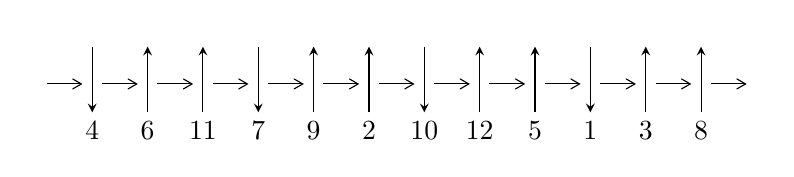
\begin{tikzpicture}[x=20pt, y=17pt]
	% nodes
	\node (C0) at (0, 0) {};
	\node (C1) at (1, 0) {};
	\node (C1U) at (1, +1) {};
	\node (C1D) at (1, -1) {4};

	\node (C2) at (2, 0) {};
	\node (C2U) at (2, +1) {};
	\node (C2D) at (2, -1) {6};

	\node (C3) at (3, 0) {};
	\node (C3U) at (3, +1) {};
	\node (C3D) at (3, -1) {11};

	\node (C4) at (4, 0) {};
	\node (C4U) at (4, +1) {};
	\node (C4D) at (4, -1) {7};

	\node (C5) at (5, 0) {};
	\node (C5U) at (5, +1) {};
	\node (C5D) at (5, -1) {9};

	\node (C6) at (6, 0) {};
	\node (C6U) at (6, +1) {};
	\node (C6D) at (6, -1) {2};

	\node (C7) at (7, 0) {};
	\node (C7U) at (7, +1) {};
	\node (C7D) at (7, -1) {10};

	\node (C8) at (8, 0) {};
	\node (C8U) at (8, +1) {};
	\node (C8D) at (8, -1) {12};

	\node (C9) at (9, 0) {};
	\node (C9U) at (9, +1) {};
	\node (C9D) at (9, -1) {5};

	\node (C10) at (10, 0) {};
	\node (C10U) at (10, +1) {};
	\node (C10D) at (10, -1) {1};

	\node (C11) at (11, 0) {};
	\node (C11U) at (11, +1) {};
	\node (C11D) at (11, -1) {3};

	\node (C12) at (12, 0) {};
	\node (C12U) at (12, +1) {};
	\node (C12D) at (12, -1) {8};
	\node (C13) at (13, 0) {};

	% arrows
	\draw[->,>={angle 60}]
	(C0) edge (C1) (C1) edge (C2) (C2) edge (C3) (C3) edge (C4) (C4) edge (C5) (C5) edge (C6) (C6) edge (C7) (C7) edge (C8) (C8) edge (C9) (C9) edge (C10) (C10) edge (C11) (C11) edge (C12) (C12) edge (C13) ;	\draw[->,>=stealth]
	(C1U) edge (C1D) (C2D) edge (C2U) (C3D) edge (C3U) (C4U) edge (C4D) (C5D) edge (C5U) (C6D) edge (C6U) (C7U) edge (C7D) (C8D) edge (C8U) (C9D) edge (C9U) (C10U) edge (C10D) (C11D) edge (C11U) (C12D) edge (C12U) ;
	\end{tikzpicture} \\
\hhline{~~} \\& 
\textbf{Solving Sequence} \\ \cline{2-2} 
 &
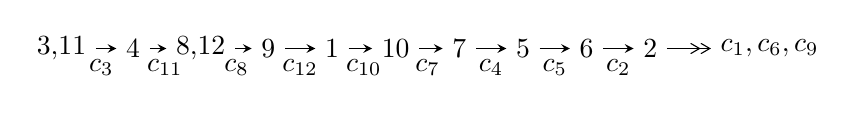
\begin{tikzpicture}[x=23pt, y=7pt]
	% node
	\node (A0) at (-1/8, 0) {3,11};
	\node (A1) at (1, 0) {4};
	\node (A2) at (33/16, 0) {8,12};
	\node (A3) at (25/8, 0) {9};
	\node (A4) at (33/8, 0) {1};
	\node (A5) at (41/8, 0) {10};
	\node (A6) at (49/8, 0) {7};
	\node (A7) at (57/8, 0) {5};
	\node (A8) at (65/8, 0) {6};
	\node (A9) at (73/8, 0) {2};
	\node (C1) at (1/2, -1) {$c_{3}$};
	\node (C2) at (3/2, -1) {$c_{11}$};
	\node (C3) at (21/8, -1) {$c_{8}$};
	\node (C4) at (29/8, -1) {$c_{12}$};
	\node (C5) at (37/8, -1) {$c_{10}$};
	\node (C6) at (45/8, -1) {$c_{7}$};
	\node (C7) at (53/8, -1) {$c_{4}$};
	\node (C8) at (61/8, -1) {$c_{5}$};
	\node (C9) at (69/8, -1) {$c_{2}$};
	\node (A10) at (11, 0) {$c_{1},c_{6},c_{9}$};

	% edge
	\draw[->,>=stealth]	
	(A0) edge (A1) (A1) edge (A2) (A2) edge (A3) (A3) edge (A4) (A4) edge (A5) (A5) edge (A6) (A6) edge (A7) (A7) edge (A8) (A8) edge (A9) ;
	\draw[->>,>={angle 60}]	
	(A9) edge (A10);
\end{tikzpicture} \\ 

\end{tabular} \\

\footnotetext{
The image of knot diagram is generated by the software ``\textbf{Draw programme}" developed by Andrew Bartholomew(\url{http://www.layer8.co.uk/maths/draw/index.htm\#Running-draw}), where we modified some parts for our purpose(\url{https://github.com/CATsTAILs/LinksPainter}).
}\phantom \\ \newline 
\centering \textbf{Ideals for irreducible components\footnotemark of $X_{\text{par}}$} 
 
\begin{align*}
I^u_{1}&=\langle 
- u^6+u^5-3 u^4+2 u^3-4 u^2+b+4 u-2,\;- u^6+u^5-3 u^4+2 u^3-4 u^2+a+4 u-1,\\
\phantom{I^u_{1}}&\phantom{= \langle  }u^8-2 u^7+5 u^6-6 u^5+9 u^4-10 u^3+8 u^2-4 u+1\rangle \\
I^u_{2}&=\langle 
4 u^{14} a- u^{14}+\cdots+8 b-6,\;4 u^{14} a- u^{14}+\cdots+4 a+4,\;u^{15}+2 u^{14}+\cdots-2 u-2\rangle \\
I^u_{3}&=\langle 
-1.77260\times10^{28} u^{29}+1.42417\times10^{29} u^{28}+\cdots+2.16558\times10^{29} b+4.09260\times10^{29},\\
\phantom{I^u_{3}}&\phantom{= \langle  }1.02276\times10^{29} u^{29}-4.13857\times10^{29} u^{28}+\cdots+4.65600\times10^{30} a-8.84106\times10^{30},\\
\phantom{I^u_{3}}&\phantom{= \langle  }u^{30}-8 u^{29}+\cdots-148 u+43\rangle \\
I^u_{4}&=\langle 
-32051170 u^{19}+10432934 u^{18}+\cdots+12423084 b-29249775,\\
\phantom{I^u_{4}}&\phantom{= \langle  }-32051170 u^{19}+10432934 u^{18}+\cdots+12423084 a-16826691,\;2 u^{20}+11 u^{18}+\cdots+4 u+1\rangle \\
I^u_{5}&=\langle 
-25516394 u^{19}+1505498 u^{18}+\cdots+12423084 b-14885617,\\
\phantom{I^u_{5}}&\phantom{= \langle  }-32363894 u^{19}+11810374 u^{18}+\cdots+6211542 a-28830039,\;2 u^{20}+11 u^{18}+\cdots+4 u+1\rangle \\
I^u_{6}&=\langle 
2 u^6 a+3 u^5 a+5 u^6+8 u^4 a+6 u^5+7 u^3 a+17 u^4+12 u^2 a+16 u^3+6 a u+18 u^2+6 b- a+15 u+2,\\
\phantom{I^u_{6}}&\phantom{= \langle  }- u^6 a- u^5 a-4 u^4 a-3 u^3 a+u^4-5 u^2 a+a^2-2 a u+2 u^2+1,\;u^7+u^6+4 u^5+3 u^4+5 u^3+3 u^2+u+1\rangle \\
I^u_{7}&=\langle 
177 u^{13}-1117 u^{12}+\cdots+52 b-1064,\;296 u^{13}-1867 u^{12}+\cdots+52 a-1718,\\
\phantom{I^u_{7}}&\phantom{= \langle  }u^{14}-7 u^{13}+\cdots-20 u+4\rangle \\
I^u_{8}&=\langle 
b- a-1,\;a^2+a u- a+u,\;u^2+u+1\rangle \\
I^u_{9}&=\langle 
-2 u^3-4 u^2+4 b-3 u+1,\;2 u^3+2 a+u-3,\;2 u^4+2 u^3+3 u^2+1\rangle \\
I^u_{10}&=\langle 
-2 u^3+8 u^2+4 b+13 u+7,\;-2 u^3+8 u^2+4 a+13 u+11,\;2 u^4+2 u^3+3 u^2+1\rangle \\
\end{align*}\\
\begin{align*}
I^u_{11}&=\langle 
u^{11}-2 u^{10}+6 u^9-7 u^8+11 u^7-7 u^6+4 u^5- u^4-5 u^3-2 u^2+2 b-2 u-2,\\
\phantom{I^u_{11}}&\phantom{= \langle  }5 u^{11}-11 u^{10}+32 u^9-39 u^8+60 u^7-43 u^6+31 u^5-12 u^4-16 u^3-12 u^2+4 a-8 u-16,\\
\phantom{I^u_{11}}&\phantom{= \langle  }u^{12}-3 u^{11}+8 u^{10}-13 u^9+18 u^8-19 u^7+13 u^6-8 u^5-2 u^4+2 u^3+4\rangle \\
I^u_{12}&=\langle 
973497 u^{11} a+1110148 u^{11}+\cdots+28861189 a-48376404,\\
\phantom{I^u_{12}}&\phantom{= \langle  }2096423 u^{11} a+1944076 u^{11}+\cdots+42713350 a+16958187,\\
\phantom{I^u_{12}}&\phantom{= \langle  }u^{12}+4 u^{11}+14 u^{10}+31 u^9+68 u^8+107 u^7+166 u^6+189 u^5+205 u^4+163 u^3+110 u^2+52 u+17\rangle \\
I^u_{13}&=\langle 
u^2+b,\;u^2+a+1,\;u^4- u^3+3 u^2-2 u+1\rangle \\
I^u_{14}&=\langle 
b- a- u,\;a^2+2 a u+a-2,\;u^2+u+1\rangle \\
\\
\end{align*}
\raggedright * 14 irreducible components of $\dim_{\mathbb{C}}=0$, with total 192 representations.\\
\footnotetext{All coefficients of polynomials are rational numbers. But the coefficients are sometimes approximated in decimal forms when there is not enough margin.}
\newpage
\renewcommand{\arraystretch}{1}
\centering \section*{I. $I^u_{1}= \langle - u^6+u^5-3 u^4+2 u^3-4 u^2+b+4 u-2,\;- u^6+u^5-3 u^4+2 u^3-4 u^2+a+4 u-1,\;u^8-2 u^7+\cdots-4 u+1 \rangle$}
\flushleft \textbf{(i) Arc colorings}\\
\begin{tabular}{m{7pt} m{180pt} m{7pt} m{180pt} }
\flushright $a_{3}=$&$\begin{pmatrix}1\\0\end{pmatrix}$ \\
\flushright $a_{11}=$&$\begin{pmatrix}0\\u\end{pmatrix}$ \\
\flushright $a_{4}=$&$\begin{pmatrix}1\\- u^2\end{pmatrix}$ \\
\flushright $a_{8}=$&$\begin{pmatrix}u^6- u^5+3 u^4-2 u^3+4 u^2-4 u+1\\u^6- u^5+3 u^4-2 u^3+4 u^2-4 u+2\end{pmatrix}$ \\
\flushright $a_{12}=$&$\begin{pmatrix}u\\u\end{pmatrix}$ \\
\flushright $a_{9}=$&$\begin{pmatrix}u^6- u^5+3 u^4-2 u^3+5 u^2-4 u+1\\u^6- u^5+3 u^4-2 u^3+5 u^2-4 u+2\end{pmatrix}$ \\
\flushright $a_{1}=$&$\begin{pmatrix}- u^7+u^6-3 u^5+2 u^4-4 u^3+4 u^2\\- u^7+u^6-3 u^5+2 u^4-4 u^3+4 u^2- u\end{pmatrix}$ \\
\flushright $a_{10}=$&$\begin{pmatrix}u^7+2 u^5+2 u^4+2 u^3+2 u^2-4 u+2\\u^7- u^6+3 u^5- u^4+4 u^3-2 u^2+1\end{pmatrix}$ \\
\flushright $a_{7}=$&$\begin{pmatrix}u^7-3 u^6+6 u^5-9 u^4+11 u^3-14 u^2+11 u-4\\u^3+u\end{pmatrix}$ \\
\flushright $a_{5}=$&$\begin{pmatrix}- u^7+3 u^6-6 u^5+9 u^4-10 u^3+14 u^2-11 u+4\\u^7- u^6+3 u^5-2 u^4+5 u^3-4 u^2+u\end{pmatrix}$ \\
\flushright $a_{6}=$&$\begin{pmatrix}-2 u^7+4 u^6-9 u^5+11 u^4-15 u^3+18 u^2-12 u+4\\- u\end{pmatrix}$ \\
\flushright $a_{2}=$&$\begin{pmatrix}- u^6+u^5-3 u^4+2 u^3-4 u^2+4 u-1\\u^2\end{pmatrix}$\\&\end{tabular}
\flushleft \textbf{(ii) Obstruction class $= -1$}\\~\\
\flushleft \textbf{(iii) Cusp Shapes $= -12 u^7+24 u^6-56 u^5+68 u^4-92 u^3+108 u^2-72 u+28$}\\~\\
\newpage\renewcommand{\arraystretch}{1}
\flushleft \textbf{(iv) u-Polynomials at the component}\newline \\
\begin{tabular}{m{50pt}|m{274pt}}
Crossings & \hspace{64pt}u-Polynomials at each crossing \\
\hline $$\begin{aligned}c_{1},c_{4},c_{7}\\c_{10}\end{aligned}$$&$\begin{aligned}
&u^8-2 u^7- u^6+6 u^5- u^4-6 u^3+8 u^2-4 u+1
\end{aligned}$\\
\hline $$\begin{aligned}c_{2},c_{3},c_{5}\\c_{6},c_{8},c_{9}\\c_{11},c_{12}\end{aligned}$$&$\begin{aligned}
&u^8-2 u^7+5 u^6-6 u^5+9 u^4-10 u^3+8 u^2-4 u+1
\end{aligned}$\\
\hline
\end{tabular}\\~\\
\newpage\renewcommand{\arraystretch}{1}
\flushleft \textbf{(v) Riley Polynomials at the component}\newline \\
\begin{tabular}{m{50pt}|m{274pt}}
Crossings & \hspace{64pt}Riley Polynomials at each crossing \\
\hline $$\begin{aligned}c_{1},c_{4},c_{7}\\c_{10}\end{aligned}$$&$\begin{aligned}
&y^8-6 y^7+23 y^6-42 y^5+43 y^4-6 y^3+14 y^2+1
\end{aligned}$\\
\hline $$\begin{aligned}c_{2},c_{3},c_{5}\\c_{6},c_{8},c_{9}\\c_{11},c_{12}\end{aligned}$$&$\begin{aligned}
&y^8+6 y^7+19 y^6+30 y^5+27 y^4+6 y^3+2 y^2+1
\end{aligned}$\\
\hline
\end{tabular}\\~\\
\newpage\flushleft \textbf{(vi) Complex Volumes and Cusp Shapes}
$$\begin{array}{c|c|c}  
\text{Solutions to }I^u_{1}& \I (\text{vol} + \sqrt{-1}CS) & \text{Cusp shape}\\
 \hline 
\begin{aligned}
u &= \phantom{-}0.341045 + 0.670313 I \\
a &= -1.14930 - 1.40518 I \\
b &= -0.149303 - 1.405180 I\end{aligned}
 & -5.74556 + 5.06444 I & -6.22905 - 4.15704 I \\ \hline\begin{aligned}
u &= \phantom{-}0.341045 - 0.670313 I \\
a &= -1.14930 + 1.40518 I \\
b &= -0.149303 + 1.405180 I\end{aligned}
 & -5.74556 - 5.06444 I & -6.22905 + 4.15704 I \\ \hline\begin{aligned}
u &= -0.548152 + 1.211390 I \\
a &= \phantom{-}0.942196 - 0.385112 I \\
b &= \phantom{-}1.94220 - 0.38511 I\end{aligned}
 & -7.41391 - 7.06214 I & \phantom{-}0.57220 + 4.67413 I \\ \hline\begin{aligned}
u &= -0.548152 - 1.211390 I \\
a &= \phantom{-}0.942196 + 0.385112 I \\
b &= \phantom{-}1.94220 + 0.38511 I\end{aligned}
 & -7.41391 + 7.06214 I & \phantom{-}0.57220 - 4.67413 I \\ \hline\begin{aligned}
u &= \phantom{-}0.566503 + 0.259919 I \\
a &= -0.452212 + 0.073091 I \\
b &= \phantom{-}0.547788 + 0.073091 I\end{aligned}
 & \phantom{-}1.156280 + 0.316293 I & \phantom{-}9.01033 - 1.88379 I \\ \hline\begin{aligned}
u &= \phantom{-}0.566503 - 0.259919 I \\
a &= -0.452212 - 0.073091 I \\
b &= \phantom{-}0.547788 - 0.073091 I\end{aligned}
 & \phantom{-}1.156280 - 0.316293 I & \phantom{-}9.01033 + 1.88379 I \\ \hline\begin{aligned}
u &= \phantom{-}0.64060 + 1.47097 I \\
a &= \phantom{-}1.65932 + 0.19565 I \\
b &= \phantom{-}2.65932 + 0.19565 I\end{aligned}
 & -14.3158 + 20.3233 I & -3.35347 - 9.42778 I \\ \hline\begin{aligned}
u &= \phantom{-}0.64060 - 1.47097 I \\
a &= \phantom{-}1.65932 - 0.19565 I \\
b &= \phantom{-}2.65932 - 0.19565 I\end{aligned}
 & -14.3158 - 20.3233 I & -3.35347 + 9.42778 I\\
 \hline 
 \end{array}$$\newpage\newpage\renewcommand{\arraystretch}{1}
\centering \section*{II. $I^u_{2}= \langle 4 u^{14} a- u^{14}+\cdots+8 b-6,\;4 u^{14} a- u^{14}+\cdots+4 a+4,\;u^{15}+2 u^{14}+\cdots-2 u-2 \rangle$}
\flushleft \textbf{(i) Arc colorings}\\
\begin{tabular}{m{7pt} m{180pt} m{7pt} m{180pt} }
\flushright $a_{3}=$&$\begin{pmatrix}1\\0\end{pmatrix}$ \\
\flushright $a_{11}=$&$\begin{pmatrix}0\\u\end{pmatrix}$ \\
\flushright $a_{4}=$&$\begin{pmatrix}1\\- u^2\end{pmatrix}$ \\
\flushright $a_{8}=$&$\begin{pmatrix}a\\-\frac{1}{2} u^{14} a+\frac{1}{8} u^{14}+\cdots+3 u+\frac{3}{4}\end{pmatrix}$ \\
\flushright $a_{12}=$&$\begin{pmatrix}u\\u\end{pmatrix}$ \\
\flushright $a_{9}=$&$\begin{pmatrix}\frac{1}{2} u^{14} a-\frac{3}{8} u^{14}+\cdots+a-\frac{5}{4}\\-\frac{1}{4} u^{14}-\frac{1}{4} u^{13}+\cdots+2 u-\frac{1}{2}\end{pmatrix}$ \\
\flushright $a_{1}=$&$\begin{pmatrix}\frac{1}{8} u^{14} a+\frac{3}{8} u^{14}+\cdots-\frac{1}{4} a-\frac{3}{4}\\\frac{1}{2} u^{14} a-\frac{1}{4} u^{14}+\cdots+a-\frac{3}{2}\end{pmatrix}$ \\
\flushright $a_{10}=$&$\begin{pmatrix}\frac{1}{2} u^{14} a-\frac{5}{8} u^{14}+\cdots+a+\frac{1}{4}\\\frac{1}{2} u^{14} a-\frac{5}{8} u^{14}+\cdots+2 u+\frac{1}{4}\end{pmatrix}$ \\
\flushright $a_{7}=$&$\begin{pmatrix}-\frac{7}{8} u^{14} a+\frac{9}{8} u^{14}+\cdots+\frac{7}{4} a-\frac{1}{4}\\-\frac{1}{2} u^{14} a+u^{14}+\cdots+a+u\end{pmatrix}$ \\
\flushright $a_{5}=$&$\begin{pmatrix}\frac{3}{4} u^{14}+\frac{5}{4} u^{13}+\cdots-\frac{1}{2} u+\frac{3}{2}\\\frac{1}{2} u^{13} a+\frac{3}{8} u^{14}+\cdots- a-\frac{3}{4}\end{pmatrix}$ \\
\flushright $a_{6}=$&$\begin{pmatrix}\frac{1}{2} u^{13} a-\frac{1}{8} u^{14}+\cdots- a+\frac{9}{4}\\\frac{1}{2} u^{13} a+\frac{1}{8} u^{14}+\cdots- a-\frac{1}{4}\end{pmatrix}$ \\
\flushright $a_{2}=$&$\begin{pmatrix}-\frac{1}{2} u^{14} a+\frac{5}{4} u^{14}+\cdots-\frac{9}{2} u-\frac{1}{2}\\-\frac{3}{8} u^{14} a+\frac{3}{8} u^{14}+\cdots+\frac{3}{4} a-\frac{3}{4}\end{pmatrix}$\\&\end{tabular}
\flushleft \textbf{(ii) Obstruction class $= -1$}\\~\\
\flushleft \textbf{(iii) Cusp Shapes $= u^{14}+u^{13}+7 u^{12}+3 u^{11}+13 u^{10}-11 u^9-14 u^8-58 u^7-71 u^6-81 u^5-66 u^4-26 u^3+2 u^2+16 u+14$}\\~\\
\newpage\renewcommand{\arraystretch}{1}
\flushleft \textbf{(iv) u-Polynomials at the component}\newline \\
\begin{tabular}{m{50pt}|m{274pt}}
Crossings & \hspace{64pt}u-Polynomials at each crossing \\
\hline $$\begin{aligned}c_{1},c_{4},c_{7}\\c_{10}\end{aligned}$$&$\begin{aligned}
&u^{30}-2 u^{29}+\cdots+22 u+1
\end{aligned}$\\
\hline $$\begin{aligned}c_{2},c_{6},c_{8}\\c_{12}\end{aligned}$$&$\begin{aligned}
&u^{30}-8 u^{29}+\cdots-148 u+43
\end{aligned}$\\
\hline $$\begin{aligned}c_{3},c_{5},c_{9}\\c_{11}\end{aligned}$$&$\begin{aligned}
&(u^{15}+2 u^{14}+\cdots-2 u-2)^{2}
\end{aligned}$\\
\hline
\end{tabular}\\~\\
\newpage\renewcommand{\arraystretch}{1}
\flushleft \textbf{(v) Riley Polynomials at the component}\newline \\
\begin{tabular}{m{50pt}|m{274pt}}
Crossings & \hspace{64pt}Riley Polynomials at each crossing \\
\hline $$\begin{aligned}c_{1},c_{4},c_{7}\\c_{10}\end{aligned}$$&$\begin{aligned}
&y^{30}-18 y^{29}+\cdots-206 y+1
\end{aligned}$\\
\hline $$\begin{aligned}c_{2},c_{6},c_{8}\\c_{12}\end{aligned}$$&$\begin{aligned}
&y^{30}+16 y^{29}+\cdots+1144 y+1849
\end{aligned}$\\
\hline $$\begin{aligned}c_{3},c_{5},c_{9}\\c_{11}\end{aligned}$$&$\begin{aligned}
&(y^{15}+16 y^{14}+\cdots-32 y-4)^{2}
\end{aligned}$\\
\hline
\end{tabular}\\~\\
\newpage\flushleft \textbf{(vi) Complex Volumes and Cusp Shapes}
$$\begin{array}{c|c|c}  
\text{Solutions to }I^u_{2}& \I (\text{vol} + \sqrt{-1}CS) & \text{Cusp shape}\\
 \hline 
\begin{aligned}
u &= -0.784607 + 0.130638 I \\
a &= \phantom{-}0.350326 - 0.122670 I \\
b &= -0.439042 - 0.323007 I\end{aligned}
 & -1.36431 + 3.70005 I & \phantom{-}4.97943 - 3.63821 I \\ \hline\begin{aligned}
u &= -0.784607 + 0.130638 I \\
a &= -0.12761 + 1.99961 I \\
b &= -0.455331 + 0.530841 I\end{aligned}
 & -1.36431 + 3.70005 I & \phantom{-}4.97943 - 3.63821 I \\ \hline\begin{aligned}
u &= -0.784607 - 0.130638 I \\
a &= \phantom{-}0.350326 + 0.122670 I \\
b &= -0.439042 + 0.323007 I\end{aligned}
 & -1.36431 - 3.70005 I & \phantom{-}4.97943 + 3.63821 I \\ \hline\begin{aligned}
u &= -0.784607 - 0.130638 I \\
a &= -0.12761 - 1.99961 I \\
b &= -0.455331 - 0.530841 I\end{aligned}
 & -1.36431 - 3.70005 I & \phantom{-}4.97943 + 3.63821 I \\ \hline\begin{aligned}
u &= \phantom{-}0.013344 + 1.238380 I \\
a &= \phantom{-}0.482542 + 0.420194 I \\
b &= \phantom{-}0.083565 - 0.439251 I\end{aligned}
 & -9.63722 - 1.22028 I & -4.95246 + 1.57507 I \\ \hline\begin{aligned}
u &= \phantom{-}0.013344 + 1.238380 I \\
a &= \phantom{-}1.32269 + 0.59357 I \\
b &= \phantom{-}2.47269 + 0.15514 I\end{aligned}
 & -9.63722 - 1.22028 I & -4.95246 + 1.57507 I \\ \hline\begin{aligned}
u &= \phantom{-}0.013344 - 1.238380 I \\
a &= \phantom{-}0.482542 - 0.420194 I \\
b &= \phantom{-}0.083565 + 0.439251 I\end{aligned}
 & -9.63722 + 1.22028 I & -4.95246 - 1.57507 I \\ \hline\begin{aligned}
u &= \phantom{-}0.013344 - 1.238380 I \\
a &= \phantom{-}1.32269 - 0.59357 I \\
b &= \phantom{-}2.47269 - 0.15514 I\end{aligned}
 & -9.63722 + 1.22028 I & -4.95246 - 1.57507 I \\ \hline\begin{aligned}
u &= -0.520579 + 1.217160 I \\
a &= \phantom{-}0.310968 - 1.284780 I \\
b &= \phantom{-}0.120416 - 0.985660 I\end{aligned}
 & -9.00480 - 3.51911 I & -6.70931 + 3.75254 I \\ \hline\begin{aligned}
u &= -0.520579 + 1.217160 I \\
a &= \phantom{-}1.41643 - 0.01039 I \\
b &= \phantom{-}2.34549 - 0.39766 I\end{aligned}
 & -9.00480 - 3.51911 I & -6.70931 + 3.75254 I\\
 \hline 
 \end{array}$$\newpage$$\begin{array}{c|c|c}  
\text{Solutions to }I^u_{2}& \I (\text{vol} + \sqrt{-1}CS) & \text{Cusp shape}\\
 \hline 
\begin{aligned}
u &= -0.520579 - 1.217160 I \\
a &= \phantom{-}0.310968 + 1.284780 I \\
b &= \phantom{-}0.120416 + 0.985660 I\end{aligned}
 & -9.00480 + 3.51911 I & -6.70931 - 3.75254 I \\ \hline\begin{aligned}
u &= -0.520579 - 1.217160 I \\
a &= \phantom{-}1.41643 + 0.01039 I \\
b &= \phantom{-}2.34549 + 0.39766 I\end{aligned}
 & -9.00480 + 3.51911 I & -6.70931 - 3.75254 I \\ \hline\begin{aligned}
u &= \phantom{-}0.261916 + 1.297730 I \\
a &= \phantom{-}0.020854 - 0.716031 I \\
b &= \phantom{-}0.182845 + 0.396366 I\end{aligned}
 & -4.42818 + 0.58231 I & \phantom{-}0.85328 - 2.04557 I \\ \hline\begin{aligned}
u &= \phantom{-}0.261916 + 1.297730 I \\
a &= -1.40607 - 0.80438 I \\
b &= -2.21703 - 0.91007 I\end{aligned}
 & -4.42818 + 0.58231 I & \phantom{-}0.85328 - 2.04557 I \\ \hline\begin{aligned}
u &= \phantom{-}0.261916 - 1.297730 I \\
a &= \phantom{-}0.020854 + 0.716031 I \\
b &= \phantom{-}0.182845 - 0.396366 I\end{aligned}
 & -4.42818 - 0.58231 I & \phantom{-}0.85328 + 2.04557 I \\ \hline\begin{aligned}
u &= \phantom{-}0.261916 - 1.297730 I \\
a &= -1.40607 + 0.80438 I \\
b &= -2.21703 + 0.91007 I\end{aligned}
 & -4.42818 - 0.58231 I & \phantom{-}0.85328 + 2.04557 I \\ \hline\begin{aligned}
u &= \phantom{-}0.585635\phantom{ +0.000000I} \\
a &= \phantom{-}0.23172 + 2.31597 I \\
b &= \phantom{-}0.989112 + 0.591455 I\end{aligned}
 & -3.88049\phantom{ +0.000000I} & \phantom{-}1.05620\phantom{ +0.000000I} \\ \hline\begin{aligned}
u &= \phantom{-}0.585635\phantom{ +0.000000I} \\
a &= \phantom{-}0.23172 - 2.31597 I \\
b &= \phantom{-}0.989112 - 0.591455 I\end{aligned}
 & -3.88049\phantom{ +0.000000I} & \phantom{-}1.05620\phantom{ +0.000000I} \\ \hline\begin{aligned}
u &= -0.43937 + 1.41900 I \\
a &= -0.136932 + 0.381950 I \\
b &= -0.399054 - 0.558077 I\end{aligned}
 & -9.7235 - 13.1451 I & -2.87381 + 8.00014 I \\ \hline\begin{aligned}
u &= -0.43937 + 1.41900 I \\
a &= -1.83297 + 0.18088 I \\
b &= -2.83221 + 0.11599 I\end{aligned}
 & -9.7235 - 13.1451 I & -2.87381 + 8.00014 I\\
 \hline 
 \end{array}$$\newpage$$\begin{array}{c|c|c}  
\text{Solutions to }I^u_{2}& \I (\text{vol} + \sqrt{-1}CS) & \text{Cusp shape}\\
 \hline 
\begin{aligned}
u &= -0.43937 - 1.41900 I \\
a &= -0.136932 - 0.381950 I \\
b &= -0.399054 + 0.558077 I\end{aligned}
 & -9.7235 + 13.1451 I & -2.87381 - 8.00014 I \\ \hline\begin{aligned}
u &= -0.43937 - 1.41900 I \\
a &= -1.83297 - 0.18088 I \\
b &= -2.83221 - 0.11599 I\end{aligned}
 & -9.7235 + 13.1451 I & -2.87381 - 8.00014 I \\ \hline\begin{aligned}
u &= \phantom{-}0.035691 + 0.462074 I \\
a &= -0.047221 - 0.354434 I \\
b &= -0.399260 + 1.160460 I\end{aligned}
 & \phantom{-}0.93924 + 2.34318 I & \phantom{-}11.9184 + 9.2243 I \\ \hline\begin{aligned}
u &= \phantom{-}0.035691 + 0.462074 I \\
a &= -1.88888 + 1.66026 I \\
b &= -0.014065 + 0.524425 I\end{aligned}
 & \phantom{-}0.93924 + 2.34318 I & \phantom{-}11.9184 + 9.2243 I \\ \hline\begin{aligned}
u &= \phantom{-}0.035691 - 0.462074 I \\
a &= -0.047221 + 0.354434 I \\
b &= -0.399260 - 1.160460 I\end{aligned}
 & \phantom{-}0.93924 - 2.34318 I & \phantom{-}11.9184 - 9.2243 I \\ \hline\begin{aligned}
u &= \phantom{-}0.035691 - 0.462074 I \\
a &= -1.88888 - 1.66026 I \\
b &= -0.014065 - 0.524425 I\end{aligned}
 & \phantom{-}0.93924 - 2.34318 I & \phantom{-}11.9184 - 9.2243 I \\ \hline\begin{aligned}
u &= \phantom{-}0.14079 + 1.54845 I \\
a &= -1.080100 + 0.342845 I \\
b &= -2.23176 - 0.04950 I\end{aligned}
 & -15.8339 + 5.3491 I & -7.74364 - 3.13359 I \\ \hline\begin{aligned}
u &= \phantom{-}0.14079 + 1.54845 I \\
a &= \phantom{-}1.88425 - 0.16237 I \\
b &= \phantom{-}2.79363 - 0.26921 I\end{aligned}
 & -15.8339 + 5.3491 I & -7.74364 - 3.13359 I \\ \hline\begin{aligned}
u &= \phantom{-}0.14079 - 1.54845 I \\
a &= -1.080100 - 0.342845 I \\
b &= -2.23176 + 0.04950 I\end{aligned}
 & -15.8339 - 5.3491 I & -7.74364 + 3.13359 I \\ \hline\begin{aligned}
u &= \phantom{-}0.14079 - 1.54845 I \\
a &= \phantom{-}1.88425 + 0.16237 I \\
b &= \phantom{-}2.79363 + 0.26921 I\end{aligned}
 & -15.8339 - 5.3491 I & -7.74364 + 3.13359 I\\
 \hline 
 \end{array}$$\newpage\newpage\renewcommand{\arraystretch}{1}
\centering \section*{III. $I^u_{3}= \langle -1.77\times10^{28} u^{29}+1.42\times10^{29} u^{28}+\cdots+2.17\times10^{29} b+4.09\times10^{29},\;1.02\times10^{29} u^{29}-4.14\times10^{29} u^{28}+\cdots+4.66\times10^{30} a-8.84\times10^{30},\;u^{30}-8 u^{29}+\cdots-148 u+43 \rangle$}
\flushleft \textbf{(i) Arc colorings}\\
\begin{tabular}{m{7pt} m{180pt} m{7pt} m{180pt} }
\flushright $a_{3}=$&$\begin{pmatrix}1\\0\end{pmatrix}$ \\
\flushright $a_{11}=$&$\begin{pmatrix}0\\u\end{pmatrix}$ \\
\flushright $a_{4}=$&$\begin{pmatrix}1\\- u^2\end{pmatrix}$ \\
\flushright $a_{8}=$&$\begin{pmatrix}-0.0219666 u^{29}+0.0888867 u^{28}+\cdots+0.298145 u+1.89885\\0.0818533 u^{29}-0.657640 u^{28}+\cdots+9.92980 u-1.88984\end{pmatrix}$ \\
\flushright $a_{12}=$&$\begin{pmatrix}u\\u\end{pmatrix}$ \\
\flushright $a_{9}=$&$\begin{pmatrix}-0.0321478 u^{29}+0.0808101 u^{28}+\cdots+8.27059 u-1.71451\\0.0716720 u^{29}-0.665717 u^{28}+\cdots+17.9022 u-5.50320\end{pmatrix}$ \\
\flushright $a_{1}=$&$\begin{pmatrix}-0.0704699 u^{29}+0.550645 u^{28}+\cdots-8.18718 u+4.94852\\-0.0379149 u^{29}+0.345413 u^{28}+\cdots-6.57038 u+2.46631\end{pmatrix}$ \\
\flushright $a_{10}=$&$\begin{pmatrix}-0.0366426 u^{29}+0.259362 u^{28}+\cdots-6.63127 u+4.11399\\0.0300022 u^{29}-0.243000 u^{28}+\cdots+3.11454 u+0.123136\end{pmatrix}$ \\
\flushright $a_{7}=$&$\begin{pmatrix}0.0280214 u^{29}-0.381962 u^{28}+\cdots+17.7589 u-8.40340\\0.154881 u^{29}-1.25831 u^{28}+\cdots+21.8368 u-8.10010\end{pmatrix}$ \\
\flushright $a_{5}=$&$\begin{pmatrix}0.104726 u^{29}-0.766133 u^{28}+\cdots-0.915910 u+2.40284\\-0.0946306 u^{29}+0.749606 u^{28}+\cdots-18.9034 u+10.2528\end{pmatrix}$ \\
\flushright $a_{6}=$&$\begin{pmatrix}0.0439498 u^{29}-0.269745 u^{28}+\cdots-6.25999 u+3.42523\\-0.0840317 u^{29}+0.682435 u^{28}+\cdots-11.5766 u+4.46425\end{pmatrix}$ \\
\flushright $a_{2}=$&$\begin{pmatrix}-0.0573560 u^{29}+0.420933 u^{28}+\cdots-2.70616 u+1.91831\\-0.0552081 u^{29}+0.398971 u^{28}+\cdots-2.33592 u+1.39986\end{pmatrix}$\\&\end{tabular}
\flushleft \textbf{(ii) Obstruction class $= -1$}\\~\\
\flushleft \textbf{(iii) Cusp Shapes $= -0.444120 u^{29}+3.62226 u^{28}+\cdots-75.2699 u+36.1756$}\\~\\
\newpage\renewcommand{\arraystretch}{1}
\flushleft \textbf{(iv) u-Polynomials at the component}\newline \\
\begin{tabular}{m{50pt}|m{274pt}}
Crossings & \hspace{64pt}u-Polynomials at each crossing \\
\hline $$\begin{aligned}c_{1},c_{4},c_{7}\\c_{10}\end{aligned}$$&$\begin{aligned}
&u^{30}-2 u^{29}+\cdots+22 u+1
\end{aligned}$\\
\hline $$\begin{aligned}c_{2},c_{6},c_{8}\\c_{12}\end{aligned}$$&$\begin{aligned}
&(u^{15}+2 u^{14}+\cdots-2 u-2)^{2}
\end{aligned}$\\
\hline $$\begin{aligned}c_{3},c_{5},c_{9}\\c_{11}\end{aligned}$$&$\begin{aligned}
&u^{30}-8 u^{29}+\cdots-148 u+43
\end{aligned}$\\
\hline
\end{tabular}\\~\\
\newpage\renewcommand{\arraystretch}{1}
\flushleft \textbf{(v) Riley Polynomials at the component}\newline \\
\begin{tabular}{m{50pt}|m{274pt}}
Crossings & \hspace{64pt}Riley Polynomials at each crossing \\
\hline $$\begin{aligned}c_{1},c_{4},c_{7}\\c_{10}\end{aligned}$$&$\begin{aligned}
&y^{30}-18 y^{29}+\cdots-206 y+1
\end{aligned}$\\
\hline $$\begin{aligned}c_{2},c_{6},c_{8}\\c_{12}\end{aligned}$$&$\begin{aligned}
&(y^{15}+16 y^{14}+\cdots-32 y-4)^{2}
\end{aligned}$\\
\hline $$\begin{aligned}c_{3},c_{5},c_{9}\\c_{11}\end{aligned}$$&$\begin{aligned}
&y^{30}+16 y^{29}+\cdots+1144 y+1849
\end{aligned}$\\
\hline
\end{tabular}\\~\\
\newpage\flushleft \textbf{(vi) Complex Volumes and Cusp Shapes}
$$\begin{array}{c|c|c}  
\text{Solutions to }I^u_{3}& \I (\text{vol} + \sqrt{-1}CS) & \text{Cusp shape}\\
 \hline 
\begin{aligned}
u &= \phantom{-}0.591752 + 0.825766 I \\
a &= -0.404241 + 0.288042 I \\
b &= -0.014065 + 0.524425 I\end{aligned}
 & \phantom{-}0.93924 + 2.34318 I & \phantom{-}11.9184 + 9.2243 I \\ \hline\begin{aligned}
u &= \phantom{-}0.591752 - 0.825766 I \\
a &= -0.404241 - 0.288042 I \\
b &= -0.014065 - 0.524425 I\end{aligned}
 & \phantom{-}0.93924 - 2.34318 I & \phantom{-}11.9184 - 9.2243 I \\ \hline\begin{aligned}
u &= -0.075236 + 1.080100 I \\
a &= -1.00453 + 1.06811 I \\
b &= -2.21703 + 0.91007 I\end{aligned}
 & -4.42818 - 0.58231 I & \phantom{-}0.85328 + 2.04557 I \\ \hline\begin{aligned}
u &= -0.075236 - 1.080100 I \\
a &= -1.00453 - 1.06811 I \\
b &= -2.21703 - 0.91007 I\end{aligned}
 & -4.42818 + 0.58231 I & \phantom{-}0.85328 - 2.04557 I \\ \hline\begin{aligned}
u &= \phantom{-}0.443554 + 1.009940 I \\
a &= \phantom{-}0.775618 - 0.105347 I \\
b &= \phantom{-}0.989112 - 0.591455 I\end{aligned}
 & -3.88049\phantom{ +0.000000I} & \phantom{-}                -6
1.056179 + 0. 10   I\phantom{ +0.000000I} \\ \hline\begin{aligned}
u &= \phantom{-}0.443554 - 1.009940 I \\
a &= \phantom{-}0.775618 + 0.105347 I \\
b &= \phantom{-}0.989112 + 0.591455 I\end{aligned}
 & -3.88049\phantom{ +0.000000I} & \phantom{-}                -6
1.056179 + 0. 10   I\phantom{ +0.000000I} \\ \hline\begin{aligned}
u &= \phantom{-}1.059000 + 0.505555 I \\
a &= \phantom{-}0.52794 + 1.39650 I \\
b &= \phantom{-}0.083565 + 0.439251 I\end{aligned}
 & -9.63722 + 1.22028 I & -4.95246 - 1.57507 I \\ \hline\begin{aligned}
u &= \phantom{-}1.059000 - 0.505555 I \\
a &= \phantom{-}0.52794 - 1.39650 I \\
b &= \phantom{-}0.083565 - 0.439251 I\end{aligned}
 & -9.63722 - 1.22028 I & -4.95246 + 1.57507 I \\ \hline\begin{aligned}
u &= \phantom{-}0.449007 + 1.109600 I \\
a &= -0.310623 - 0.117713 I \\
b &= -0.455331 + 0.530841 I\end{aligned}
 & -1.36431 + 3.70005 I & \phantom{-}4.97943 - 3.63821 I \\ \hline\begin{aligned}
u &= \phantom{-}0.449007 - 1.109600 I \\
a &= -0.310623 + 0.117713 I \\
b &= -0.455331 - 0.530841 I\end{aligned}
 & -1.36431 - 3.70005 I & \phantom{-}4.97943 + 3.63821 I\\
 \hline 
 \end{array}$$\newpage$$\begin{array}{c|c|c}  
\text{Solutions to }I^u_{3}& \I (\text{vol} + \sqrt{-1}CS) & \text{Cusp shape}\\
 \hline 
\begin{aligned}
u &= -0.712558 + 0.108600 I \\
a &= -0.25372 - 1.78675 I \\
b &= -0.399260 - 1.160460 I\end{aligned}
 & \phantom{-}0.93924 - 2.34318 I & \phantom{-}11.9184 - 9.2243 I \\ \hline\begin{aligned}
u &= -0.712558 - 0.108600 I \\
a &= -0.25372 + 1.78675 I \\
b &= -0.399260 + 1.160460 I\end{aligned}
 & \phantom{-}0.93924 + 2.34318 I & \phantom{-}11.9184 + 9.2243 I \\ \hline\begin{aligned}
u &= -0.012294 + 1.332420 I \\
a &= \phantom{-}1.42848 - 0.77990 I \\
b &= \phantom{-}2.34549 - 0.39766 I\end{aligned}
 & -9.00480 - 3.51911 I & -6.70931 + 3.75254 I \\ \hline\begin{aligned}
u &= -0.012294 - 1.332420 I \\
a &= \phantom{-}1.42848 + 0.77990 I \\
b &= \phantom{-}2.34549 + 0.39766 I\end{aligned}
 & -9.00480 + 3.51911 I & -6.70931 - 3.75254 I \\ \hline\begin{aligned}
u &= \phantom{-}0.645515 + 0.054065 I \\
a &= \phantom{-}0.751134 - 0.625068 I \\
b &= -0.439042 - 0.323007 I\end{aligned}
 & -1.36431 + 3.70005 I & \phantom{-}4.97943 - 3.63821 I \\ \hline\begin{aligned}
u &= \phantom{-}0.645515 - 0.054065 I \\
a &= \phantom{-}0.751134 + 0.625068 I \\
b &= -0.439042 + 0.323007 I\end{aligned}
 & -1.36431 - 3.70005 I & \phantom{-}4.97943 + 3.63821 I \\ \hline\begin{aligned}
u &= \phantom{-}0.29345 + 1.39308 I \\
a &= \phantom{-}1.70894 - 0.39664 I \\
b &= \phantom{-}2.79363 - 0.26921 I\end{aligned}
 & -15.8339 + 5.3491 I & -7.74364 - 3.13359 I \\ \hline\begin{aligned}
u &= \phantom{-}0.29345 - 1.39308 I \\
a &= \phantom{-}1.70894 + 0.39664 I \\
b &= \phantom{-}2.79363 + 0.26921 I\end{aligned}
 & -15.8339 - 5.3491 I & -7.74364 + 3.13359 I \\ \hline\begin{aligned}
u &= \phantom{-}1.44906 + 0.04107 I \\
a &= -0.12382 - 1.54513 I \\
b &= -0.399054 - 0.558077 I\end{aligned}
 & -9.7235 - 13.1451 I & -2.87381 + 8.00014 I \\ \hline\begin{aligned}
u &= \phantom{-}1.44906 - 0.04107 I \\
a &= -0.12382 + 1.54513 I \\
b &= -0.399054 + 0.558077 I\end{aligned}
 & -9.7235 + 13.1451 I & -2.87381 - 8.00014 I\\
 \hline 
 \end{array}$$\newpage$$\begin{array}{c|c|c}  
\text{Solutions to }I^u_{3}& \I (\text{vol} + \sqrt{-1}CS) & \text{Cusp shape}\\
 \hline 
\begin{aligned}
u &= \phantom{-}0.53111 + 1.38940 I \\
a &= -1.83564 - 0.05128 I \\
b &= -2.83221 - 0.11599 I\end{aligned}
 & -9.7235 + 13.1451 I & -2.87381 - 8.00014 I \\ \hline\begin{aligned}
u &= \phantom{-}0.53111 - 1.38940 I \\
a &= -1.83564 + 0.05128 I \\
b &= -2.83221 + 0.11599 I\end{aligned}
 & -9.7235 - 13.1451 I & -2.87381 + 8.00014 I \\ \hline\begin{aligned}
u &= -1.40117 + 0.50158 I \\
a &= \phantom{-}0.054654 + 1.276660 I \\
b &= \phantom{-}0.182845 + 0.396366 I\end{aligned}
 & -4.42818 + 0.58231 I & \phantom{-}0.85328 - 2.04557 I \\ \hline\begin{aligned}
u &= -1.40117 - 0.50158 I \\
a &= \phantom{-}0.054654 - 1.276660 I \\
b &= \phantom{-}0.182845 - 0.396366 I\end{aligned}
 & -4.42818 - 0.58231 I & \phantom{-}0.85328 + 2.04557 I \\ \hline\begin{aligned}
u &= \phantom{-}0.55829 + 1.41828 I \\
a &= \phantom{-}1.71347 - 0.13431 I \\
b &= \phantom{-}2.47269 + 0.15514 I\end{aligned}
 & -9.63722 - 1.22028 I & -4.95246 + 1.57507 I \\ \hline\begin{aligned}
u &= \phantom{-}0.55829 - 1.41828 I \\
a &= \phantom{-}1.71347 + 0.13431 I \\
b &= \phantom{-}2.47269 - 0.15514 I\end{aligned}
 & -9.63722 + 1.22028 I & -4.95246 - 1.57507 I \\ \hline\begin{aligned}
u &= -0.264872 + 0.387644 I \\
a &= \phantom{-}1.63538 - 1.39243 I \\
b &= \phantom{-}0.120416 + 0.985660 I\end{aligned}
 & -9.00480 + 3.51911 I & -6.70931 - 3.75254 I \\ \hline\begin{aligned}
u &= -0.264872 - 0.387644 I \\
a &= \phantom{-}1.63538 + 1.39243 I \\
b &= \phantom{-}0.120416 - 0.985660 I\end{aligned}
 & -9.00480 - 3.51911 I & -6.70931 + 3.75254 I \\ \hline\begin{aligned}
u &= \phantom{-}0.44538 + 1.83853 I \\
a &= -1.45375 + 0.31455 I \\
b &= -2.23176 + 0.04950 I\end{aligned}
 & -15.8339 - 5.3491 I & \phantom{-0.000000 } 0 \\ \hline\begin{aligned}
u &= \phantom{-}0.44538 - 1.83853 I \\
a &= -1.45375 - 0.31455 I \\
b &= -2.23176 - 0.04950 I\end{aligned}
 & -15.8339 + 5.3491 I & \phantom{-0.000000 } 0\\
 \hline 
 \end{array}$$\newpage\newpage\renewcommand{\arraystretch}{1}
\centering \section*{IV. $I^u_{4}= \langle -3.21\times10^{7} u^{19}+1.04\times10^{7} u^{18}+\cdots+1.24\times10^{7} b-2.92\times10^{7},\;-3.21\times10^{7} u^{19}+1.04\times10^{7} u^{18}+\cdots+1.24\times10^{7} a-1.68\times10^{7},\;2 u^{20}+11 u^{18}+\cdots+4 u+1 \rangle$}
\flushleft \textbf{(i) Arc colorings}\\
\begin{tabular}{m{7pt} m{180pt} m{7pt} m{180pt} }
\flushright $a_{3}=$&$\begin{pmatrix}1\\0\end{pmatrix}$ \\
\flushright $a_{11}=$&$\begin{pmatrix}0\\u\end{pmatrix}$ \\
\flushright $a_{4}=$&$\begin{pmatrix}1\\- u^2\end{pmatrix}$ \\
\flushright $a_{8}=$&$\begin{pmatrix}2.57997 u^{19}-0.839802 u^{18}+\cdots+5.83982 u+1.35447\\2.57997 u^{19}-0.839802 u^{18}+\cdots+5.83982 u+2.35447\end{pmatrix}$ \\
\flushright $a_{12}=$&$\begin{pmatrix}u\\u\end{pmatrix}$ \\
\flushright $a_{9}=$&$\begin{pmatrix}2.57997 u^{19}-0.839802 u^{18}+\cdots+5.83982 u+1.35447\\2.57997 u^{19}-0.839802 u^{18}+\cdots+5.83982 u+2.35447\end{pmatrix}$ \\
\flushright $a_{1}=$&$\begin{pmatrix}0.839802 u^{19}+0.560480 u^{18}+\cdots+4.80547 u+1.28998\\0.839802 u^{19}+0.560480 u^{18}+\cdots+3.80547 u+1.28998\end{pmatrix}$ \\
\flushright $a_{10}=$&$\begin{pmatrix}-2.75425 u^{19}+1.12237 u^{18}+\cdots-0.266870 u+0.439076\\-1.80815 u^{19}+2.12100 u^{18}+\cdots+2.27399 u+0.719316\end{pmatrix}$ \\
\flushright $a_{7}=$&$\begin{pmatrix}0.368104 u^{19}+0.851099 u^{18}+\cdots+1.54512 u+0.318890\\1.07331 u^{19}+1.27931 u^{18}+\cdots+5.66065 u+2.13487\end{pmatrix}$ \\
\flushright $a_{5}=$&$\begin{pmatrix}-2.33263 u^{19}+4.14232 u^{18}+\cdots+1.61849 u-0.565148\\0.0638148 u^{19}+2.08837 u^{18}+\cdots+2.36860 u-0.271319\end{pmatrix}$ \\
\flushright $a_{6}=$&$\begin{pmatrix}-2.39644 u^{19}+2.05395 u^{18}+\cdots-0.750113 u-0.293830\\-1.78017 u^{19}+0.847531 u^{18}+\cdots-2.86952 u-1.57817\end{pmatrix}$ \\
\flushright $a_{2}=$&$\begin{pmatrix}0.946107 u^{19}+0.998631 u^{18}+\cdots+2.54086 u+0.280240\\1.82394 u^{19}+0.0731794 u^{18}+\cdots+4.73492 u+1.50906\end{pmatrix}$\\&\end{tabular}
\flushleft \textbf{(ii) Obstruction class $= -1$}\\~\\
\flushleft \textbf{(iii) Cusp Shapes $= -\frac{201044}{3105771} u^{19}-\frac{4918603}{3105771} u^{18}+\cdots-\frac{11843897}{1035257} u+\frac{24068461}{6211542}$}\\~\\
\newpage\renewcommand{\arraystretch}{1}
\flushleft \textbf{(iv) u-Polynomials at the component}\newline \\
\begin{tabular}{m{50pt}|m{274pt}}
Crossings & \hspace{64pt}u-Polynomials at each crossing \\
\hline $$\begin{aligned}c_{1},c_{7}\end{aligned}$$&$\begin{aligned}
&(u^{10}+2 u^9+u^8-2 u^7-3 u^6+2 u^4+2 u^3-3 u^2-2 u-2)^2
\end{aligned}$\\
\hline $$\begin{aligned}c_{2},c_{3},c_{5}\\c_{6},c_{8},c_{9}\\c_{11},c_{12}\end{aligned}$$&$\begin{aligned}
&2(2 u^{20}+11 u^{18}+\cdots+4 u+1)
\end{aligned}$\\
\hline $$\begin{aligned}c_{4},c_{10}\end{aligned}$$&$\begin{aligned}
&4(4 u^{20}-28 u^{19}+\cdots-448 u+73)
\end{aligned}$\\
\hline
\end{tabular}\\~\\
\newpage\renewcommand{\arraystretch}{1}
\flushleft \textbf{(v) Riley Polynomials at the component}\newline \\
\begin{tabular}{m{50pt}|m{274pt}}
Crossings & \hspace{64pt}Riley Polynomials at each crossing \\
\hline $$\begin{aligned}c_{1},c_{7}\end{aligned}$$&$\begin{aligned}
&(y^{10}-2 y^9+3 y^8-6 y^7- y^6-6 y^5+10 y^4-4 y^3+9 y^2+8 y+4)^2
\end{aligned}$\\
\hline $$\begin{aligned}c_{2},c_{3},c_{5}\\c_{6},c_{8},c_{9}\\c_{11},c_{12}\end{aligned}$$&$\begin{aligned}
&4(4 y^{20}+44 y^{19}+\cdots-6 y+1)
\end{aligned}$\\
\hline $$\begin{aligned}c_{4},c_{10}\end{aligned}$$&$\begin{aligned}
&16(16 y^{20}-8 y^{19}+\cdots+42678 y+5329)
\end{aligned}$\\
\hline
\end{tabular}\\~\\
\newpage\flushleft \textbf{(vi) Complex Volumes and Cusp Shapes}
$$\begin{array}{c|c|c}  
\text{Solutions to }I^u_{4}& \I (\text{vol} + \sqrt{-1}CS) & \text{Cusp shape}\\
 \hline 
\begin{aligned}
u &= \phantom{-}0.863041 + 0.424455 I \\
a &= \phantom{-}0.150300 - 0.336990 I \\
b &= \phantom{-}1.150300 - 0.336990 I\end{aligned}
 & -1.77310 + 4.32568 I & \phantom{-}2.37801 - 5.30660 I \\ \hline\begin{aligned}
u &= \phantom{-}0.863041 - 0.424455 I \\
a &= \phantom{-}0.150300 + 0.336990 I \\
b &= \phantom{-}1.150300 + 0.336990 I\end{aligned}
 & -1.77310 - 4.32568 I & \phantom{-}2.37801 + 5.30660 I \\ \hline\begin{aligned}
u &= \phantom{-}0.532247 + 0.733699 I \\
a &= \phantom{-}0.094270 - 0.781019 I \\
b &= \phantom{-}1.094270 - 0.781019 I\end{aligned}
 & -3.96232\phantom{ +0.000000I} & \phantom{-}2.14246 + 0. I\phantom{ +0.000000I} \\ \hline\begin{aligned}
u &= \phantom{-}0.532247 - 0.733699 I \\
a &= \phantom{-}0.094270 + 0.781019 I \\
b &= \phantom{-}1.094270 + 0.781019 I\end{aligned}
 & -3.96232\phantom{ +0.000000I} & \phantom{-}2.14246 + 0. I\phantom{ +0.000000I} \\ \hline\begin{aligned}
u &= -0.854424 + 0.268587 I \\
a &= \phantom{-}0.208143 - 1.003220 I \\
b &= \phantom{-}1.20814 - 1.00322 I\end{aligned}
 & -4.52678 - 8.23619 I & \phantom{-}1.62263 + 8.93292 I \\ \hline\begin{aligned}
u &= -0.854424 - 0.268587 I \\
a &= \phantom{-}0.208143 + 1.003220 I \\
b &= \phantom{-}1.20814 + 1.00322 I\end{aligned}
 & -4.52678 + 8.23619 I & \phantom{-}1.62263 - 8.93292 I \\ \hline\begin{aligned}
u &= -0.294566 + 0.835743 I \\
a &= -1.091400 + 0.492363 I \\
b &= -0.091403 + 0.492363 I\end{aligned}
 & -7.15291\phantom{ +0.000000I} & -10.64039 + 0. I\phantom{ +0.000000I} \\ \hline\begin{aligned}
u &= -0.294566 - 0.835743 I \\
a &= -1.091400 - 0.492363 I \\
b &= -0.091403 - 0.492363 I\end{aligned}
 & -7.15291\phantom{ +0.000000I} & -10.64039 + 0. I\phantom{ +0.000000I} \\ \hline\begin{aligned}
u &= -0.219333 + 1.144070 I \\
a &= \phantom{-}1.97577 + 0.10621 I \\
b &= \phantom{-}2.97577 + 0.10621 I\end{aligned}
 & -1.77310 - 4.32568 I & \phantom{-}2.37801 + 5.30660 I \\ \hline\begin{aligned}
u &= -0.219333 - 1.144070 I \\
a &= \phantom{-}1.97577 - 0.10621 I \\
b &= \phantom{-}2.97577 - 0.10621 I\end{aligned}
 & -1.77310 + 4.32568 I & \phantom{-}2.37801 - 5.30660 I\\
 \hline 
 \end{array}$$\newpage$$\begin{array}{c|c|c}  
\text{Solutions to }I^u_{4}& \I (\text{vol} + \sqrt{-1}CS) & \text{Cusp shape}\\
 \hline 
\begin{aligned}
u &= \phantom{-}0.482255 + 0.664266 I \\
a &= -0.579450 + 0.348965 I \\
b &= \phantom{-}0.420550 + 0.348965 I\end{aligned}
 & \phantom{-}0.97046 + 1.97408 I & \phantom{-}9.55166 - 2.43496 I \\ \hline\begin{aligned}
u &= \phantom{-}0.482255 - 0.664266 I \\
a &= -0.579450 - 0.348965 I \\
b &= \phantom{-}0.420550 - 0.348965 I\end{aligned}
 & \phantom{-}0.97046 - 1.97408 I & \phantom{-}9.55166 + 2.43496 I \\ \hline\begin{aligned}
u &= -0.365634 + 1.127630 I \\
a &= \phantom{-}0.27691 - 1.63768 I \\
b &= \phantom{-}1.27691 - 1.63768 I\end{aligned}
 & -10.4971 - 10.3444 I & -5.80333 + 10.34256 I \\ \hline\begin{aligned}
u &= -0.365634 - 1.127630 I \\
a &= \phantom{-}0.27691 + 1.63768 I \\
b &= \phantom{-}1.27691 + 1.63768 I\end{aligned}
 & -10.4971 + 10.3444 I & -5.80333 - 10.34256 I \\ \hline\begin{aligned}
u &= -0.445937 + 1.170140 I \\
a &= \phantom{-}2.03642 - 0.41858 I \\
b &= \phantom{-}3.03642 - 0.41858 I\end{aligned}
 & -4.52678 - 8.23619 I & \phantom{-}1.62263 + 8.93292 I \\ \hline\begin{aligned}
u &= -0.445937 - 1.170140 I \\
a &= \phantom{-}2.03642 + 0.41858 I \\
b &= \phantom{-}3.03642 + 0.41858 I\end{aligned}
 & -4.52678 + 8.23619 I & \phantom{-}1.62263 - 8.93292 I \\ \hline\begin{aligned}
u &= -0.387590 + 0.116004 I \\
a &= -0.92490 + 1.07958 I \\
b &= \phantom{-}0.075100 + 1.079580 I\end{aligned}
 & \phantom{-}0.97046 + 1.97408 I & \phantom{-}9.55166 - 2.43496 I \\ \hline\begin{aligned}
u &= -0.387590 - 0.116004 I \\
a &= -0.92490 - 1.07958 I \\
b &= \phantom{-}0.075100 - 1.079580 I\end{aligned}
 & \phantom{-}0.97046 - 1.97408 I & \phantom{-}9.55166 + 2.43496 I \\ \hline\begin{aligned}
u &= \phantom{-}0.68994 + 1.64040 I \\
a &= \phantom{-}1.353940 + 0.198723 I \\
b &= \phantom{-}2.35394 + 0.19872 I\end{aligned}
 & -10.4971 + 10.3444 I & -5.80333 - 10.34256 I \\ \hline\begin{aligned}
u &= \phantom{-}0.68994 - 1.64040 I \\
a &= \phantom{-}1.353940 - 0.198723 I \\
b &= \phantom{-}2.35394 - 0.19872 I\end{aligned}
 & -10.4971 - 10.3444 I & -5.80333 + 10.34256 I\\
 \hline 
 \end{array}$$\newpage\newpage\renewcommand{\arraystretch}{1}
\centering \section*{V. $I^u_{5}= \langle -2.55\times10^{7} u^{19}+1.51\times10^{6} u^{18}+\cdots+1.24\times10^{7} b-1.49\times10^{7},\;-3.24\times10^{7} u^{19}+1.18\times10^{7} u^{18}+\cdots+6.21\times10^{6} a-2.88\times10^{7},\;2 u^{20}+11 u^{18}+\cdots+4 u+1 \rangle$}
\flushleft \textbf{(i) Arc colorings}\\
\begin{tabular}{m{7pt} m{180pt} m{7pt} m{180pt} }
\flushright $a_{3}=$&$\begin{pmatrix}1\\0\end{pmatrix}$ \\
\flushright $a_{11}=$&$\begin{pmatrix}0\\u\end{pmatrix}$ \\
\flushright $a_{4}=$&$\begin{pmatrix}1\\- u^2\end{pmatrix}$ \\
\flushright $a_{8}=$&$\begin{pmatrix}5.21028 u^{19}-1.90136 u^{18}+\cdots+9.08615 u+4.64137\\2.05395 u^{19}-0.121186 u^{18}+\cdots+4.49906 u+1.19822\end{pmatrix}$ \\
\flushright $a_{12}=$&$\begin{pmatrix}u\\u\end{pmatrix}$ \\
\flushright $a_{9}=$&$\begin{pmatrix}4.36275 u^{19}-1.87619 u^{18}+\cdots+7.10397 u+3.75128\\1.20642 u^{19}-0.0960206 u^{18}+\cdots+2.51688 u+0.308135\end{pmatrix}$ \\
\flushright $a_{1}=$&$\begin{pmatrix}-2.01949 u^{19}-0.106305 u^{18}+\cdots-6.22944 u-1.77437\\0.998631 u^{19}-1.93025 u^{18}+\cdots-1.61197 u-0.473054\end{pmatrix}$ \\
\flushright $a_{10}=$&$\begin{pmatrix}2.08425 u^{19}-1.02147 u^{18}+\cdots+4.71094 u+2.53696\\0.428211 u^{19}-1.79215 u^{18}+\cdots+0.405560 u-0.352605\end{pmatrix}$ \\
\flushright $a_{7}=$&$\begin{pmatrix}5.54874 u^{19}-2.01949 u^{18}+\cdots+11.7767 u+4.86805\\u^3+u\end{pmatrix}$ \\
\flushright $a_{5}=$&$\begin{pmatrix}-2.61627 u^{19}+1.20642 u^{18}+\cdots-2.88059 u-2.71566\\-0.925452 u^{19}+0.450391 u^{18}+\cdots-0.526847 u-0.438917\end{pmatrix}$ \\
\flushright $a_{6}=$&$\begin{pmatrix}-4.70894 u^{19}+2.57997 u^{18}+\cdots-7.97120 u-3.57806\\- u\end{pmatrix}$ \\
\flushright $a_{2}=$&$\begin{pmatrix}-2.57997 u^{19}+0.839802 u^{18}+\cdots-5.83982 u-1.35447\\u^2\end{pmatrix}$\\&\end{tabular}
\flushleft \textbf{(ii) Obstruction class $= -1$}\\~\\
\flushleft \textbf{(iii) Cusp Shapes $= -\frac{201044}{3105771} u^{19}-\frac{4918603}{3105771} u^{18}+\cdots-\frac{11843897}{1035257} u+\frac{24068461}{6211542}$}\\~\\
\newpage\renewcommand{\arraystretch}{1}
\flushleft \textbf{(iv) u-Polynomials at the component}\newline \\
\begin{tabular}{m{50pt}|m{274pt}}
Crossings & \hspace{64pt}u-Polynomials at each crossing \\
\hline $$\begin{aligned}c_{1},c_{7}\end{aligned}$$&$\begin{aligned}
&4(4 u^{20}-28 u^{19}+\cdots-448 u+73)
\end{aligned}$\\
\hline $$\begin{aligned}c_{2},c_{3},c_{5}\\c_{6},c_{8},c_{9}\\c_{11},c_{12}\end{aligned}$$&$\begin{aligned}
&2(2 u^{20}+11 u^{18}+\cdots+4 u+1)
\end{aligned}$\\
\hline $$\begin{aligned}c_{4},c_{10}\end{aligned}$$&$\begin{aligned}
&(u^{10}+2 u^9+u^8-2 u^7-3 u^6+2 u^4+2 u^3-3 u^2-2 u-2)^2
\end{aligned}$\\
\hline
\end{tabular}\\~\\
\newpage\renewcommand{\arraystretch}{1}
\flushleft \textbf{(v) Riley Polynomials at the component}\newline \\
\begin{tabular}{m{50pt}|m{274pt}}
Crossings & \hspace{64pt}Riley Polynomials at each crossing \\
\hline $$\begin{aligned}c_{1},c_{7}\end{aligned}$$&$\begin{aligned}
&16(16 y^{20}-8 y^{19}+\cdots+42678 y+5329)
\end{aligned}$\\
\hline $$\begin{aligned}c_{2},c_{3},c_{5}\\c_{6},c_{8},c_{9}\\c_{11},c_{12}\end{aligned}$$&$\begin{aligned}
&4(4 y^{20}+44 y^{19}+\cdots-6 y+1)
\end{aligned}$\\
\hline $$\begin{aligned}c_{4},c_{10}\end{aligned}$$&$\begin{aligned}
&(y^{10}-2 y^9+3 y^8-6 y^7- y^6-6 y^5+10 y^4-4 y^3+9 y^2+8 y+4)^2
\end{aligned}$\\
\hline
\end{tabular}\\~\\
\newpage\flushleft \textbf{(vi) Complex Volumes and Cusp Shapes}
$$\begin{array}{c|c|c}  
\text{Solutions to }I^u_{5}& \I (\text{vol} + \sqrt{-1}CS) & \text{Cusp shape}\\
 \hline 
\begin{aligned}
u &= \phantom{-}0.863041 + 0.424455 I \\
a &= \phantom{-}0.485394 + 0.775205 I \\
b &= -0.244227 - 0.191588 I\end{aligned}
 & -1.77310 + 4.32568 I & \phantom{-}2.37801 - 5.30660 I \\ \hline\begin{aligned}
u &= \phantom{-}0.863041 - 0.424455 I \\
a &= \phantom{-}0.485394 - 0.775205 I \\
b &= -0.244227 + 0.191588 I\end{aligned}
 & -1.77310 - 4.32568 I & \phantom{-}2.37801 + 5.30660 I \\ \hline\begin{aligned}
u &= \phantom{-}0.532247 + 0.733699 I \\
a &= \phantom{-}1.44676 + 0.95061 I \\
b &= \phantom{-}1.13636\phantom{ +0.000000I}\end{aligned}
 & -3.96232\phantom{ +0.000000I} & \phantom{-}2.14246 + 0. I\phantom{ +0.000000I} \\ \hline\begin{aligned}
u &= \phantom{-}0.532247 - 0.733699 I \\
a &= \phantom{-}1.44676 - 0.95061 I \\
b &= \phantom{-}1.13636\phantom{ +0.000000I}\end{aligned}
 & -3.96232\phantom{ +0.000000I} & \phantom{-}2.14246 + 0. I\phantom{ +0.000000I} \\ \hline\begin{aligned}
u &= -0.854424 + 0.268587 I \\
a &= -0.30663 + 1.50788 I \\
b &= \phantom{-}0.560140 + 0.410838 I\end{aligned}
 & -4.52678 - 8.23619 I & \phantom{-}1.62263 + 8.93292 I \\ \hline\begin{aligned}
u &= -0.854424 - 0.268587 I \\
a &= -0.30663 - 1.50788 I \\
b &= \phantom{-}0.560140 - 0.410838 I\end{aligned}
 & -4.52678 + 8.23619 I & \phantom{-}1.62263 - 8.93292 I \\ \hline\begin{aligned}
u &= -0.294566 + 0.835743 I \\
a &= -2.23987 - 0.62703 I \\
b &= -3.01887\phantom{ +0.000000I}\end{aligned}
 & -7.15291\phantom{ +0.000000I} & -10.64039 + 0. I\phantom{ +0.000000I} \\ \hline\begin{aligned}
u &= -0.294566 - 0.835743 I \\
a &= -2.23987 + 0.62703 I \\
b &= -3.01887\phantom{ +0.000000I}\end{aligned}
 & -7.15291\phantom{ +0.000000I} & -10.64039 + 0. I\phantom{ +0.000000I} \\ \hline\begin{aligned}
u &= -0.219333 + 1.144070 I \\
a &= \phantom{-}0.253117 + 0.850599 I \\
b &= -0.244227 + 0.191588 I\end{aligned}
 & -1.77310 - 4.32568 I & \phantom{-}2.37801 + 5.30660 I \\ \hline\begin{aligned}
u &= -0.219333 - 1.144070 I \\
a &= \phantom{-}0.253117 - 0.850599 I \\
b &= -0.244227 - 0.191588 I\end{aligned}
 & -1.77310 + 4.32568 I & \phantom{-}2.37801 - 5.30660 I\\
 \hline 
 \end{array}$$\newpage$$\begin{array}{c|c|c}  
\text{Solutions to }I^u_{5}& \I (\text{vol} + \sqrt{-1}CS) & \text{Cusp shape}\\
 \hline 
\begin{aligned}
u &= \phantom{-}0.482255 + 0.664266 I \\
a &= -0.071592 + 0.163124 I \\
b &= -0.234632 + 0.628244 I\end{aligned}
 & \phantom{-}0.97046 + 1.97408 I & \phantom{-}9.55166 - 2.43496 I \\ \hline\begin{aligned}
u &= \phantom{-}0.482255 - 0.664266 I \\
a &= -0.071592 - 0.163124 I \\
b &= -0.234632 - 0.628244 I\end{aligned}
 & \phantom{-}0.97046 - 1.97408 I & \phantom{-}9.55166 + 2.43496 I \\ \hline\begin{aligned}
u &= -0.365634 + 1.127630 I \\
a &= -1.144170 + 0.105482 I \\
b &= -2.64003 - 0.02134 I\end{aligned}
 & -10.4971 - 10.3444 I & -5.80333 + 10.34256 I \\ \hline\begin{aligned}
u &= -0.365634 - 1.127630 I \\
a &= -1.144170 - 0.105482 I \\
b &= -2.64003 + 0.02134 I\end{aligned}
 & -10.4971 + 10.3444 I & -5.80333 - 10.34256 I \\ \hline\begin{aligned}
u &= -0.445937 + 1.170140 I \\
a &= \phantom{-}0.116733 - 0.150369 I \\
b &= \phantom{-}0.560140 + 0.410838 I\end{aligned}
 & -4.52678 - 8.23619 I & \phantom{-}1.62263 + 8.93292 I \\ \hline\begin{aligned}
u &= -0.445937 - 1.170140 I \\
a &= \phantom{-}0.116733 + 0.150369 I \\
b &= \phantom{-}0.560140 - 0.410838 I\end{aligned}
 & -4.52678 + 8.23619 I & \phantom{-}1.62263 - 8.93292 I \\ \hline\begin{aligned}
u &= -0.387590 + 0.116004 I \\
a &= \phantom{-}0.43654 + 2.54296 I \\
b &= -0.234632 + 0.628244 I\end{aligned}
 & \phantom{-}0.97046 + 1.97408 I & \phantom{-}9.55166 - 2.43496 I \\ \hline\begin{aligned}
u &= -0.387590 - 0.116004 I \\
a &= \phantom{-}0.43654 - 2.54296 I \\
b &= -0.234632 - 0.628244 I\end{aligned}
 & \phantom{-}0.97046 - 1.97408 I & \phantom{-}9.55166 + 2.43496 I \\ \hline\begin{aligned}
u &= \phantom{-}0.68994 + 1.64040 I \\
a &= -1.97628 + 0.07761 I \\
b &= -2.64003 + 0.02134 I\end{aligned}
 & -10.4971 + 10.3444 I & -5.80333 - 10.34256 I \\ \hline\begin{aligned}
u &= \phantom{-}0.68994 - 1.64040 I \\
a &= -1.97628 - 0.07761 I \\
b &= -2.64003 - 0.02134 I\end{aligned}
 & -10.4971 - 10.3444 I & -5.80333 + 10.34256 I\\
 \hline 
 \end{array}$$\newpage\newpage\renewcommand{\arraystretch}{1}
\centering \section*{VI. $I^u_{6}= \langle 2 u^6 a+5 u^6+\cdots- a+2,\;- u^6 a- u^5 a+\cdots+a^2+1,\;u^7+u^6+4 u^5+3 u^4+5 u^3+3 u^2+u+1 \rangle$}
\flushleft \textbf{(i) Arc colorings}\\
\begin{tabular}{m{7pt} m{180pt} m{7pt} m{180pt} }
\flushright $a_{3}=$&$\begin{pmatrix}1\\0\end{pmatrix}$ \\
\flushright $a_{11}=$&$\begin{pmatrix}0\\u\end{pmatrix}$ \\
\flushright $a_{4}=$&$\begin{pmatrix}1\\- u^2\end{pmatrix}$ \\
\flushright $a_{8}=$&$\begin{pmatrix}a\\-\frac{1}{3} u^6 a-\frac{5}{6} u^6+\cdots+\frac{1}{6} a-\frac{1}{3}\end{pmatrix}$ \\
\flushright $a_{12}=$&$\begin{pmatrix}u\\u\end{pmatrix}$ \\
\flushright $a_{9}=$&$\begin{pmatrix}\frac{1}{6} u^6 a+\frac{2}{3} u^6+\cdots+\frac{7}{6} a+\frac{1}{6}\\-\frac{1}{6} u^6 a-\frac{1}{6} u^6+\cdots+\frac{1}{3} a-\frac{1}{6}\end{pmatrix}$ \\
\flushright $a_{1}=$&$\begin{pmatrix}-\frac{1}{6} u^6 a+\frac{1}{3} u^6+\cdots-\frac{7}{6} a+\frac{5}{6}\\\frac{1}{2} u^6 a+u^6+\cdots-\frac{1}{2} a+\frac{1}{2}\end{pmatrix}$ \\
\flushright $a_{10}=$&$\begin{pmatrix}- u^6 a- u^5 a-3 u^4 a-2 u^3 a-2 u^2 a- a u+a\\- u^6 a- u^5 a-3 u^4 a-2 u^3 a-2 u^2 a- a u\end{pmatrix}$ \\
\flushright $a_{7}=$&$\begin{pmatrix}\frac{2}{3} u^6 a+\frac{1}{6} u^6+\cdots+\frac{13}{6} a-\frac{1}{3}\\-\frac{1}{2} u^6 a-\frac{1}{2} u^6+\cdots+a-\frac{1}{2}\end{pmatrix}$ \\
\flushright $a_{5}=$&$\begin{pmatrix}-\frac{1}{6} u^6 a-\frac{1}{6} u^6+\cdots+\frac{4}{3} a+\frac{5}{6}\\-\frac{1}{3} u^6 a+\frac{1}{6} u^6+\cdots+\frac{1}{6} a-\frac{4}{3}\end{pmatrix}$ \\
\flushright $a_{6}=$&$\begin{pmatrix}\frac{1}{6} u^6 a-\frac{1}{3} u^6+\cdots+\frac{7}{6} a+\frac{1}{6}\\-\frac{1}{6} u^6 a-\frac{1}{6} u^6+\cdots+\frac{1}{3} a-\frac{7}{6}\end{pmatrix}$ \\
\flushright $a_{2}=$&$\begin{pmatrix}-\frac{1}{2} u^6 a-\frac{1}{2} u^6+\cdots- a+\frac{1}{2}\\\frac{1}{3} u^6 a+\frac{1}{3} u^6+\cdots-\frac{2}{3} a+\frac{1}{3}\end{pmatrix}$\\&\end{tabular}
\flushleft \textbf{(ii) Obstruction class $= 1$}\\~\\
\flushleft \textbf{(iii) Cusp Shapes $= -2 u^6-10 u^5-13 u^4-32 u^3-22 u^2-29 u-16$}\\~\\
\newpage\renewcommand{\arraystretch}{1}
\flushleft \textbf{(iv) u-Polynomials at the component}\newline \\
\begin{tabular}{m{50pt}|m{274pt}}
Crossings & \hspace{64pt}u-Polynomials at each crossing \\
\hline $$\begin{aligned}c_{1},c_{4},c_{7}\\c_{10}\end{aligned}$$&$\begin{aligned}
&u^{14}- u^{13}+\cdots-6 u+1
\end{aligned}$\\
\hline $$\begin{aligned}c_{2},c_{8}\end{aligned}$$&$\begin{aligned}
&u^{14}+7 u^{13}+\cdots+20 u+4
\end{aligned}$\\
\hline $$\begin{aligned}c_{3},c_{9}\end{aligned}$$&$\begin{aligned}
&(u^7+u^6+4 u^5+3 u^4+5 u^3+3 u^2+u+1)^2
\end{aligned}$\\
\hline $$\begin{aligned}c_{5},c_{11}\end{aligned}$$&$\begin{aligned}
&(u^7- u^6+4 u^5-3 u^4+5 u^3-3 u^2+u-1)^2
\end{aligned}$\\
\hline $$\begin{aligned}c_{6},c_{12}\end{aligned}$$&$\begin{aligned}
&u^{14}-7 u^{13}+\cdots-20 u+4
\end{aligned}$\\
\hline
\end{tabular}\\~\\
\newpage\renewcommand{\arraystretch}{1}
\flushleft \textbf{(v) Riley Polynomials at the component}\newline \\
\begin{tabular}{m{50pt}|m{274pt}}
Crossings & \hspace{64pt}Riley Polynomials at each crossing \\
\hline $$\begin{aligned}c_{1},c_{4},c_{7}\\c_{10}\end{aligned}$$&$\begin{aligned}
&y^{14}+7 y^{13}+\cdots-6 y+1
\end{aligned}$\\
\hline $$\begin{aligned}c_{2},c_{6},c_{8}\\c_{12}\end{aligned}$$&$\begin{aligned}
&y^{14}+3 y^{13}+\cdots+16 y+16
\end{aligned}$\\
\hline $$\begin{aligned}c_{3},c_{5},c_{9}\\c_{11}\end{aligned}$$&$\begin{aligned}
&(y^7+7 y^6+20 y^5+27 y^4+13 y^3-5 y^2-5 y-1)^2
\end{aligned}$\\
\hline
\end{tabular}\\~\\
\newpage\flushleft \textbf{(vi) Complex Volumes and Cusp Shapes}
$$\begin{array}{c|c|c}  
\text{Solutions to }I^u_{6}& \I (\text{vol} + \sqrt{-1}CS) & \text{Cusp shape}\\
 \hline 
\begin{aligned}
u &= -0.727632\phantom{ +0.000000I} \\
a &= \phantom{-}0.55098 + 1.42676 I \\
b &= \phantom{-}0.190731 - 0.051917 I\end{aligned}
 & -1.45874\phantom{ +0.000000I} & \phantom{-}3.88000\phantom{ +0.000000I} \\ \hline\begin{aligned}
u &= -0.727632\phantom{ +0.000000I} \\
a &= \phantom{-}0.55098 - 1.42676 I \\
b &= \phantom{-}0.190731 + 0.051917 I\end{aligned}
 & -1.45874\phantom{ +0.000000I} & \phantom{-}3.88000\phantom{ +0.000000I} \\ \hline\begin{aligned}
u &= \phantom{-}0.181669 + 1.341540 I \\
a &= \phantom{-}0.102984 + 0.460514 I \\
b &= \phantom{-}0.021966 - 0.804617 I\end{aligned}
 & -5.18918 + 0.24371 I & -8.52695 + 1.31812 I \\ \hline\begin{aligned}
u &= \phantom{-}0.181669 + 1.341540 I \\
a &= -1.38378 - 1.07006 I \\
b &= -2.13249 - 1.12742 I\end{aligned}
 & -5.18918 + 0.24371 I & -8.52695 + 1.31812 I \\ \hline\begin{aligned}
u &= \phantom{-}0.181669 - 1.341540 I \\
a &= \phantom{-}0.102984 - 0.460514 I \\
b &= \phantom{-}0.021966 + 0.804617 I\end{aligned}
 & -5.18918 - 0.24371 I & -8.52695 - 1.31812 I \\ \hline\begin{aligned}
u &= \phantom{-}0.181669 - 1.341540 I \\
a &= -1.38378 + 1.07006 I \\
b &= -2.13249 + 1.12742 I\end{aligned}
 & -5.18918 - 0.24371 I & -8.52695 - 1.31812 I \\ \hline\begin{aligned}
u &= \phantom{-}0.111545 + 0.598906 I \\
a &= -0.098390 - 0.225904 I \\
b &= \phantom{-}0.208665 - 1.320170 I\end{aligned}
 & \phantom{-}0.76719 + 2.52853 I & -9.7693 - 13.5452 I \\ \hline\begin{aligned}
u &= \phantom{-}0.111545 + 0.598906 I \\
a &= -1.31371 + 1.24073 I \\
b &= \phantom{-}0.148089 + 0.421187 I\end{aligned}
 & \phantom{-}0.76719 + 2.52853 I & -9.7693 - 13.5452 I \\ \hline\begin{aligned}
u &= \phantom{-}0.111545 - 0.598906 I \\
a &= -0.098390 + 0.225904 I \\
b &= \phantom{-}0.208665 + 1.320170 I\end{aligned}
 & \phantom{-}0.76719 - 2.52853 I & -9.7693 + 13.5452 I \\ \hline\begin{aligned}
u &= \phantom{-}0.111545 - 0.598906 I \\
a &= -1.31371 - 1.24073 I \\
b &= \phantom{-}0.148089 - 0.421187 I\end{aligned}
 & \phantom{-}0.76719 - 2.52853 I & -9.7693 + 13.5452 I\\
 \hline 
 \end{array}$$\newpage$$\begin{array}{c|c|c}  
\text{Solutions to }I^u_{6}& \I (\text{vol} + \sqrt{-1}CS) & \text{Cusp shape}\\
 \hline 
\begin{aligned}
u &= -0.42940 + 1.35504 I \\
a &= -1.291350 + 0.284587 I \\
b &= -2.47211 + 0.16468 I\end{aligned}
 & -9.65304 - 8.50275 I & -4.64372 + 5.74713 I \\ \hline\begin{aligned}
u &= -0.42940 + 1.35504 I \\
a &= \phantom{-}0.933270 - 0.968989 I \\
b &= \phantom{-}1.53514 - 0.86559 I\end{aligned}
 & -9.65304 - 8.50275 I & -4.64372 + 5.74713 I \\ \hline\begin{aligned}
u &= -0.42940 - 1.35504 I \\
a &= -1.291350 - 0.284587 I \\
b &= -2.47211 - 0.16468 I\end{aligned}
 & -9.65304 + 8.50275 I & -4.64372 - 5.74713 I \\ \hline\begin{aligned}
u &= -0.42940 - 1.35504 I \\
a &= \phantom{-}0.933270 + 0.968989 I \\
b &= \phantom{-}1.53514 + 0.86559 I\end{aligned}
 & -9.65304 + 8.50275 I & -4.64372 - 5.74713 I\\
 \hline 
 \end{array}$$\newpage\newpage\renewcommand{\arraystretch}{1}
\centering \section*{VII. $I^u_{7}= \langle 177 u^{13}-1117 u^{12}+\cdots+52 b-1064,\;296 u^{13}-1867 u^{12}+\cdots+52 a-1718,\;u^{14}-7 u^{13}+\cdots-20 u+4 \rangle$}
\flushleft \textbf{(i) Arc colorings}\\
\begin{tabular}{m{7pt} m{180pt} m{7pt} m{180pt} }
\flushright $a_{3}=$&$\begin{pmatrix}1\\0\end{pmatrix}$ \\
\flushright $a_{11}=$&$\begin{pmatrix}0\\u\end{pmatrix}$ \\
\flushright $a_{4}=$&$\begin{pmatrix}1\\- u^2\end{pmatrix}$ \\
\flushright $a_{8}=$&$\begin{pmatrix}-5.69231 u^{13}+35.9038 u^{12}+\cdots-118.846 u+33.0385\\-3.40385 u^{13}+21.4808 u^{12}+\cdots-73.0385 u+20.4615\end{pmatrix}$ \\
\flushright $a_{12}=$&$\begin{pmatrix}u\\u\end{pmatrix}$ \\
\flushright $a_{9}=$&$\begin{pmatrix}-4.69231 u^{13}+29.5577 u^{12}+\cdots-96.0769 u+26.6538\\-2.40385 u^{13}+15.1346 u^{12}+\cdots-50.2692 u+14.0769\end{pmatrix}$ \\
\flushright $a_{1}=$&$\begin{pmatrix}1.21154 u^{13}-8.11538 u^{12}+\cdots+27 u-7.57692\\0.480769 u^{13}-3.51923 u^{12}+\cdots+14.1923 u-3.38462\end{pmatrix}$ \\
\flushright $a_{10}=$&$\begin{pmatrix}-1.13462 u^{13}+7.46154 u^{12}+\cdots-25.4231 u+6.19231\\-0.173077 u^{13}+1.09615 u^{12}+\cdots-10.4231 u+2.61538\end{pmatrix}$ \\
\flushright $a_{7}=$&$\begin{pmatrix}-4.75000 u^{13}+29.8846 u^{12}+\cdots-99.0769 u+28.0385\\-1.01923 u^{13}+6.21154 u^{12}+\cdots-18.6538 u+5.53846\end{pmatrix}$ \\
\flushright $a_{5}=$&$\begin{pmatrix}-1.67308 u^{13}+10.0769 u^{12}+\cdots-25.2692 u+7.03846\\-0.403846 u^{13}+2.40385 u^{12}+\cdots-1.42308 u+0.153846\end{pmatrix}$ \\
\flushright $a_{6}=$&$\begin{pmatrix}-5.11538 u^{13}+32.4038 u^{12}+\cdots-105 u+29.2692\\-1.59615 u^{13}+10.1731 u^{12}+\cdots-33.1923 u+9.15385\end{pmatrix}$ \\
\flushright $a_{2}=$&$\begin{pmatrix}0.846154 u^{13}-5.44231 u^{12}+\cdots+10.3462 u-2.73077\\0.519231 u^{13}-3.55769 u^{12}+\cdots+10.4231 u-2.92308\end{pmatrix}$\\&\end{tabular}
\flushleft \textbf{(ii) Obstruction class $= 1$}\\~\\
\flushleft \textbf{(iii) Cusp Shapes $= -\frac{454}{13} u^{13}+\frac{2870}{13} u^{12}-\frac{9845}{13} u^{11}+\frac{23675}{13} u^{10}-\frac{42801}{13} u^9+\frac{62428}{13} u^8-\frac{76369}{13} u^7+\frac{78835}{13} u^6-\frac{71328}{13} u^5+\frac{55147}{13} u^4-\frac{37555}{13} u^3+\frac{20790}{13} u^2-\frac{9494}{13} u+\frac{2552}{13}$}\\~\\
\newpage\renewcommand{\arraystretch}{1}
\flushleft \textbf{(iv) u-Polynomials at the component}\newline \\
\begin{tabular}{m{50pt}|m{274pt}}
Crossings & \hspace{64pt}u-Polynomials at each crossing \\
\hline $$\begin{aligned}c_{1},c_{4},c_{7}\\c_{10}\end{aligned}$$&$\begin{aligned}
&u^{14}- u^{13}+\cdots-6 u+1
\end{aligned}$\\
\hline $$\begin{aligned}c_{2},c_{8}\end{aligned}$$&$\begin{aligned}
&(u^7- u^6+4 u^5-3 u^4+5 u^3-3 u^2+u-1)^2
\end{aligned}$\\
\hline $$\begin{aligned}c_{3},c_{9}\end{aligned}$$&$\begin{aligned}
&u^{14}-7 u^{13}+\cdots-20 u+4
\end{aligned}$\\
\hline $$\begin{aligned}c_{5},c_{11}\end{aligned}$$&$\begin{aligned}
&u^{14}+7 u^{13}+\cdots+20 u+4
\end{aligned}$\\
\hline $$\begin{aligned}c_{6},c_{12}\end{aligned}$$&$\begin{aligned}
&(u^7+u^6+4 u^5+3 u^4+5 u^3+3 u^2+u+1)^2
\end{aligned}$\\
\hline
\end{tabular}\\~\\
\newpage\renewcommand{\arraystretch}{1}
\flushleft \textbf{(v) Riley Polynomials at the component}\newline \\
\begin{tabular}{m{50pt}|m{274pt}}
Crossings & \hspace{64pt}Riley Polynomials at each crossing \\
\hline $$\begin{aligned}c_{1},c_{4},c_{7}\\c_{10}\end{aligned}$$&$\begin{aligned}
&y^{14}+7 y^{13}+\cdots-6 y+1
\end{aligned}$\\
\hline $$\begin{aligned}c_{2},c_{6},c_{8}\\c_{12}\end{aligned}$$&$\begin{aligned}
&(y^7+7 y^6+20 y^5+27 y^4+13 y^3-5 y^2-5 y-1)^2
\end{aligned}$\\
\hline $$\begin{aligned}c_{3},c_{5},c_{9}\\c_{11}\end{aligned}$$&$\begin{aligned}
&y^{14}+3 y^{13}+\cdots+16 y+16
\end{aligned}$\\
\hline
\end{tabular}\\~\\
\newpage\flushleft \textbf{(vi) Complex Volumes and Cusp Shapes}
$$\begin{array}{c|c|c}  
\text{Solutions to }I^u_{7}& \I (\text{vol} + \sqrt{-1}CS) & \text{Cusp shape}\\
 \hline 
\begin{aligned}
u &= -0.059064 + 1.014840 I \\
a &= -0.80465 + 1.22915 I \\
b &= -2.13249 + 1.12742 I\end{aligned}
 & -5.18918 - 0.24371 I & -8.52695 - 1.31812 I \\ \hline\begin{aligned}
u &= -0.059064 - 1.014840 I \\
a &= -0.80465 - 1.22915 I \\
b &= -2.13249 - 1.12742 I\end{aligned}
 & -5.18918 + 0.24371 I & -8.52695 + 1.31812 I \\ \hline\begin{aligned}
u &= \phantom{-}0.653886 + 0.784063 I \\
a &= -0.372401 + 0.129379 I \\
b &= \phantom{-}0.148089 + 0.421187 I\end{aligned}
 & \phantom{-}0.76719 + 2.52853 I & -9.7693 - 13.5452 I \\ \hline\begin{aligned}
u &= \phantom{-}0.653886 - 0.784063 I \\
a &= -0.372401 - 0.129379 I \\
b &= \phantom{-}0.148089 - 0.421187 I\end{aligned}
 & \phantom{-}0.76719 - 2.52853 I & -9.7693 + 13.5452 I \\ \hline\begin{aligned}
u &= \phantom{-}0.262126 + 1.075930 I \\
a &= \phantom{-}0.346261 - 0.690308 I \\
b &= \phantom{-}0.190731 - 0.051917 I\end{aligned}
 & -1.45874\phantom{ +0.000000I} & \phantom{-}3.87999 + 0. I\phantom{ +0.000000I} \\ \hline\begin{aligned}
u &= \phantom{-}0.262126 - 1.075930 I \\
a &= \phantom{-}0.346261 + 0.690308 I \\
b &= \phantom{-}0.190731 + 0.051917 I\end{aligned}
 & -1.45874\phantom{ +0.000000I} & \phantom{-}3.87999 + 0. I\phantom{ +0.000000I} \\ \hline\begin{aligned}
u &= -0.398553 + 0.771164 I \\
a &= -0.078706 - 0.588337 I \\
b &= \phantom{-}1.53514 - 0.86559 I\end{aligned}
 & -9.65304 - 8.50275 I & -4.64372 + 5.74713 I \\ \hline\begin{aligned}
u &= -0.398553 - 0.771164 I \\
a &= -0.078706 + 0.588337 I \\
b &= \phantom{-}1.53514 + 0.86559 I\end{aligned}
 & -9.65304 + 8.50275 I & -4.64372 - 5.74713 I \\ \hline\begin{aligned}
u &= \phantom{-}0.689615 + 0.061837 I \\
a &= -0.02905 - 2.16732 I \\
b &= \phantom{-}0.208665 - 1.320170 I\end{aligned}
 & \phantom{-}0.76719 + 2.52853 I & -9.7693 - 13.5452 I \\ \hline\begin{aligned}
u &= \phantom{-}0.689615 - 0.061837 I \\
a &= -0.02905 + 2.16732 I \\
b &= \phantom{-}0.208665 + 1.320170 I\end{aligned}
 & \phantom{-}0.76719 - 2.52853 I & -9.7693 + 13.5452 I\\
 \hline 
 \end{array}$$\newpage$$\begin{array}{c|c|c}  
\text{Solutions to }I^u_{7}& \I (\text{vol} + \sqrt{-1}CS) & \text{Cusp shape}\\
 \hline 
\begin{aligned}
u &= \phantom{-}0.66949 + 1.54849 I \\
a &= -1.63384 - 0.07956 I \\
b &= -2.47211 - 0.16468 I\end{aligned}
 & -9.65304 + 8.50275 I & -4.64372 - 5.74713 I \\ \hline\begin{aligned}
u &= \phantom{-}0.66949 - 1.54849 I \\
a &= -1.63384 + 0.07956 I \\
b &= -2.47211 + 0.16468 I\end{aligned}
 & -9.65304 - 8.50275 I & -4.64372 + 5.74713 I \\ \hline\begin{aligned}
u &= \phantom{-}1.68250 + 0.33852 I \\
a &= \phantom{-}0.07238 + 1.59182 I \\
b &= \phantom{-}0.021966 + 0.804617 I\end{aligned}
 & -5.18918 - 0.24371 I & -8.52695 - 1.31812 I \\ \hline\begin{aligned}
u &= \phantom{-}1.68250 - 0.33852 I \\
a &= \phantom{-}0.07238 - 1.59182 I \\
b &= \phantom{-}0.021966 - 0.804617 I\end{aligned}
 & -5.18918 + 0.24371 I & -8.52695 + 1.31812 I\\
 \hline 
 \end{array}$$\newpage\newpage\renewcommand{\arraystretch}{1}
\centering \section*{VIII. $I^u_{8}= \langle b- a-1,\;a^2+a u- a+u,\;u^2+u+1 \rangle$}
\flushleft \textbf{(i) Arc colorings}\\
\begin{tabular}{m{7pt} m{180pt} m{7pt} m{180pt} }
\flushright $a_{3}=$&$\begin{pmatrix}1\\0\end{pmatrix}$ \\
\flushright $a_{11}=$&$\begin{pmatrix}0\\u\end{pmatrix}$ \\
\flushright $a_{4}=$&$\begin{pmatrix}1\\u+1\end{pmatrix}$ \\
\flushright $a_{8}=$&$\begin{pmatrix}a\\a+1\end{pmatrix}$ \\
\flushright $a_{12}=$&$\begin{pmatrix}u\\u\end{pmatrix}$ \\
\flushright $a_{9}=$&$\begin{pmatrix}a- u-1\\a- u\end{pmatrix}$ \\
\flushright $a_{1}=$&$\begin{pmatrix}- a u+u\\- a u\end{pmatrix}$ \\
\flushright $a_{10}=$&$\begin{pmatrix}- a u- a- u+1\\- a u\end{pmatrix}$ \\
\flushright $a_{7}=$&$\begin{pmatrix}- a+2\\u+1\end{pmatrix}$ \\
\flushright $a_{5}=$&$\begin{pmatrix}2 a u+a-2 u-2\\a u+1\end{pmatrix}$ \\
\flushright $a_{6}=$&$\begin{pmatrix}a u+a-2 u-3\\- u\end{pmatrix}$ \\
\flushright $a_{2}=$&$\begin{pmatrix}a+u-1\\- u-1\end{pmatrix}$\\&\end{tabular}
\flushleft \textbf{(ii) Obstruction class $= -1$}\\~\\
\flushleft \textbf{(iii) Cusp Shapes $= 16 u+6$}\\~\\
\newpage\renewcommand{\arraystretch}{1}
\flushleft \textbf{(iv) u-Polynomials at the component}\newline \\
\begin{tabular}{m{50pt}|m{274pt}}
Crossings & \hspace{64pt}u-Polynomials at each crossing \\
\hline $$\begin{aligned}c_{1},c_{4},c_{7}\\c_{10}\end{aligned}$$&$\begin{aligned}
&u^4- u^3- u^2-2 u+4
\end{aligned}$\\
\hline $$\begin{aligned}c_{2},c_{3},c_{5}\\c_{6},c_{8},c_{9}\\c_{11},c_{12}\end{aligned}$$&$\begin{aligned}
&(u^2+u+1)^2
\end{aligned}$\\
\hline
\end{tabular}\\~\\
\newpage\renewcommand{\arraystretch}{1}
\flushleft \textbf{(v) Riley Polynomials at the component}\newline \\
\begin{tabular}{m{50pt}|m{274pt}}
Crossings & \hspace{64pt}Riley Polynomials at each crossing \\
\hline $$\begin{aligned}c_{1},c_{4},c_{7}\\c_{10}\end{aligned}$$&$\begin{aligned}
&y^4-3 y^3+5 y^2-12 y+16
\end{aligned}$\\
\hline $$\begin{aligned}c_{2},c_{3},c_{5}\\c_{6},c_{8},c_{9}\\c_{11},c_{12}\end{aligned}$$&$\begin{aligned}
&(y^2+y+1)^2
\end{aligned}$\\
\hline
\end{tabular}\\~\\
\newpage\flushleft \textbf{(vi) Complex Volumes and Cusp Shapes}
$$\begin{array}{c|c|c}  
\text{Solutions to }I^u_{8}& \I (\text{vol} + \sqrt{-1}CS) & \text{Cusp shape}\\
 \hline 
\begin{aligned}
u &= -0.500000 + 0.866025 I \\
a &= -0.395644 + 0.228425 I \\
b &= \phantom{-}0.604356 + 0.228425 I\end{aligned}
 & -4.93480 - 8.11953 I & -2.00000 + 13.85641 I \\ \hline\begin{aligned}
u &= -0.500000 + 0.866025 I \\
a &= \phantom{-}1.89564 - 1.09445 I \\
b &= \phantom{-}2.89564 - 1.09445 I\end{aligned}
 & -4.93480 - 8.11953 I & -2.00000 + 13.85641 I \\ \hline\begin{aligned}
u &= -0.500000 - 0.866025 I \\
a &= -0.395644 - 0.228425 I \\
b &= \phantom{-}0.604356 - 0.228425 I\end{aligned}
 & -4.93480 + 8.11953 I & -2.00000 - 13.85641 I \\ \hline\begin{aligned}
u &= -0.500000 - 0.866025 I \\
a &= \phantom{-}1.89564 + 1.09445 I \\
b &= \phantom{-}2.89564 + 1.09445 I\end{aligned}
 & -4.93480 + 8.11953 I & -2.00000 - 13.85641 I\\
 \hline 
 \end{array}$$\newpage\newpage\renewcommand{\arraystretch}{1}
\centering \section*{IX. $I^u_{9}= \langle -2 u^3-4 u^2+4 b-3 u+1,\;2 u^3+2 a+u-3,\;2 u^4+2 u^3+3 u^2+1 \rangle$}
\flushleft \textbf{(i) Arc colorings}\\
\begin{tabular}{m{7pt} m{180pt} m{7pt} m{180pt} }
\flushright $a_{3}=$&$\begin{pmatrix}1\\0\end{pmatrix}$ \\
\flushright $a_{11}=$&$\begin{pmatrix}0\\u\end{pmatrix}$ \\
\flushright $a_{4}=$&$\begin{pmatrix}1\\- u^2\end{pmatrix}$ \\
\flushright $a_{8}=$&$\begin{pmatrix}- u^3-\frac{1}{2} u+\frac{3}{2}\\\frac{1}{2} u^3+u^2+\frac{3}{4} u-\frac{1}{4}\end{pmatrix}$ \\
\flushright $a_{12}=$&$\begin{pmatrix}u\\u\end{pmatrix}$ \\
\flushright $a_{9}=$&$\begin{pmatrix}-\frac{3}{2} u^3- u^2-\frac{5}{4} u+\frac{7}{4}\\0\end{pmatrix}$ \\
\flushright $a_{1}=$&$\begin{pmatrix}u^3+2 u^2+\frac{7}{2} u+\frac{3}{2}\\\frac{1}{2} u^3+\frac{3}{4} u-\frac{3}{4}\end{pmatrix}$ \\
\flushright $a_{10}=$&$\begin{pmatrix}2 u^3- u-3\\-\frac{1}{2} u^3- u^2-\frac{3}{4} u+\frac{1}{4}\end{pmatrix}$ \\
\flushright $a_{7}=$&$\begin{pmatrix}u^3+\frac{1}{2} u-\frac{7}{2}\\- u^3- u\end{pmatrix}$ \\
\flushright $a_{5}=$&$\begin{pmatrix}4 u^3+6 u^2+6 u-1\\- u\end{pmatrix}$ \\
\flushright $a_{6}=$&$\begin{pmatrix}\frac{7}{2} u^3+4 u^2+\frac{13}{4} u-\frac{13}{4}\\- u\end{pmatrix}$ \\
\flushright $a_{2}=$&$\begin{pmatrix}-\frac{1}{2} u^3+2 u^2+\frac{13}{4} u+\frac{11}{4}\\u^2\end{pmatrix}$\\&\end{tabular}
\flushleft \textbf{(ii) Obstruction class $= 1$}\\~\\
\flushleft \textbf{(iii) Cusp Shapes $= -2 u^3-4 u^2-3 u-\frac{5}{2}$}\\~\\
\newpage\renewcommand{\arraystretch}{1}
\flushleft \textbf{(iv) u-Polynomials at the component}\newline \\
\begin{tabular}{m{50pt}|m{274pt}}
Crossings & \hspace{64pt}u-Polynomials at each crossing \\
\hline $$\begin{aligned}c_{1},c_{7}\end{aligned}$$&$\begin{aligned}
&4(4 u^4-15 u^2-2 u+17)
\end{aligned}$\\
\hline $$\begin{aligned}c_{2},c_{5},c_{8}\\c_{11}\end{aligned}$$&$\begin{aligned}
&2(2 u^4-2 u^3+3 u^2+1)
\end{aligned}$\\
\hline $$\begin{aligned}c_{3},c_{6},c_{9}\\c_{12}\end{aligned}$$&$\begin{aligned}
&2(2 u^4+2 u^3+3 u^2+1)
\end{aligned}$\\
\hline $$\begin{aligned}c_{4},c_{10}\end{aligned}$$&$\begin{aligned}
&(u^2-2 u+2)^2
\end{aligned}$\\
\hline
\end{tabular}\\~\\
\newpage\renewcommand{\arraystretch}{1}
\flushleft \textbf{(v) Riley Polynomials at the component}\newline \\
\begin{tabular}{m{50pt}|m{274pt}}
Crossings & \hspace{64pt}Riley Polynomials at each crossing \\
\hline $$\begin{aligned}c_{1},c_{7}\end{aligned}$$&$\begin{aligned}
&16(16 y^4-120 y^3+361 y^2-514 y+289)
\end{aligned}$\\
\hline $$\begin{aligned}c_{2},c_{3},c_{5}\\c_{6},c_{8},c_{9}\\c_{11},c_{12}\end{aligned}$$&$\begin{aligned}
&4(4 y^4+8 y^3+13 y^2+6 y+1)
\end{aligned}$\\
\hline $$\begin{aligned}c_{4},c_{10}\end{aligned}$$&$\begin{aligned}
&(y^2+4)^2
\end{aligned}$\\
\hline
\end{tabular}\\~\\
\newpage\flushleft \textbf{(vi) Complex Volumes and Cusp Shapes}
$$\begin{array}{c|c|c}  
\text{Solutions to }I^u_{9}& \I (\text{vol} + \sqrt{-1}CS) & \text{Cusp shape}\\
 \hline 
\begin{aligned}
u &= -0.637550 + 1.056350 I \\
a &= -0.056347 - 0.637550 I \\
b &= -0.500000 - 0.500000 I\end{aligned}
 & -4.93480 - 7.32772 I & -1.50000 + 2.00000 I \\ \hline\begin{aligned}
u &= -0.637550 - 1.056350 I \\
a &= -0.056347 + 0.637550 I \\
b &= -0.500000 + 0.500000 I\end{aligned}
 & -4.93480 + 7.32772 I & -1.50000 - 2.00000 I \\ \hline\begin{aligned}
u &= \phantom{-}0.137550 + 0.556347 I \\
a &= \phantom{-}1.55635 - 0.13755 I \\
b &= -0.500000 + 0.500000 I\end{aligned}
 & -4.93480 + 7.32772 I & -1.50000 - 2.00000 I \\ \hline\begin{aligned}
u &= \phantom{-}0.137550 - 0.556347 I \\
a &= \phantom{-}1.55635 + 0.13755 I \\
b &= -0.500000 - 0.500000 I\end{aligned}
 & -4.93480 - 7.32772 I & -1.50000 + 2.00000 I\\
 \hline 
 \end{array}$$\newpage\newpage\renewcommand{\arraystretch}{1}
\centering \section*{X. $I^u_{10}= \langle -2 u^3+8 u^2+4 b+13 u+7,\;-2 u^3+8 u^2+4 a+13 u+11,\;2 u^4+2 u^3+3 u^2+1 \rangle$}
\flushleft \textbf{(i) Arc colorings}\\
\begin{tabular}{m{7pt} m{180pt} m{7pt} m{180pt} }
\flushright $a_{3}=$&$\begin{pmatrix}1\\0\end{pmatrix}$ \\
\flushright $a_{11}=$&$\begin{pmatrix}0\\u\end{pmatrix}$ \\
\flushright $a_{4}=$&$\begin{pmatrix}1\\- u^2\end{pmatrix}$ \\
\flushright $a_{8}=$&$\begin{pmatrix}\frac{1}{2} u^3-2 u^2-\frac{13}{4} u-\frac{11}{4}\\\frac{1}{2} u^3-2 u^2-\frac{13}{4} u-\frac{7}{4}\end{pmatrix}$ \\
\flushright $a_{12}=$&$\begin{pmatrix}u\\u\end{pmatrix}$ \\
\flushright $a_{9}=$&$\begin{pmatrix}\frac{1}{2} u^3- u^2-\frac{13}{4} u-\frac{11}{4}\\\frac{1}{2} u^3- u^2-\frac{13}{4} u-\frac{7}{4}\end{pmatrix}$ \\
\flushright $a_{1}=$&$\begin{pmatrix}\frac{5}{2} u^3+4 u^2+\frac{15}{4} u+\frac{1}{4}\\\frac{5}{2} u^3+4 u^2+\frac{11}{4} u+\frac{1}{4}\end{pmatrix}$ \\
\flushright $a_{10}=$&$\begin{pmatrix}-\frac{7}{2} u^3-\frac{7}{2} u^2-\frac{23}{4} u+\frac{1}{2}\\-2 u^3-\frac{3}{2} u^2-\frac{7}{2} u+\frac{5}{4}\end{pmatrix}$ \\
\flushright $a_{7}=$&$\begin{pmatrix}\frac{9}{4} u^3+\frac{5}{2} u^2+\frac{31}{8} u-\frac{1}{8}\\\frac{7}{4} u^3+\frac{3}{2} u^2+\frac{17}{8} u-\frac{7}{8}\end{pmatrix}$ \\
\flushright $a_{5}=$&$\begin{pmatrix}-\frac{13}{4} u^3-\frac{11}{2} u^2-\frac{43}{8} u-\frac{3}{8}\\-\frac{11}{4} u^3-\frac{9}{2} u^2-\frac{29}{8} u+\frac{3}{8}\end{pmatrix}$ \\
\flushright $a_{6}=$&$\begin{pmatrix}\frac{1}{2} u^3+u^2+\frac{7}{4} u+\frac{3}{4}\\\frac{1}{2} u^3+u^2+\frac{7}{4} u+\frac{3}{4}\end{pmatrix}$ \\
\flushright $a_{2}=$&$\begin{pmatrix}\frac{3}{2} u^3+2 u^2+\frac{9}{4} u+\frac{3}{4}\\\frac{3}{2} u^3+2 u^2+\frac{9}{4} u-\frac{1}{4}\end{pmatrix}$\\&\end{tabular}
\flushleft \textbf{(ii) Obstruction class $= 1$}\\~\\
\flushleft \textbf{(iii) Cusp Shapes $= -2 u^3-4 u^2-3 u-\frac{5}{2}$}\\~\\
\newpage\renewcommand{\arraystretch}{1}
\flushleft \textbf{(iv) u-Polynomials at the component}\newline \\
\begin{tabular}{m{50pt}|m{274pt}}
Crossings & \hspace{64pt}u-Polynomials at each crossing \\
\hline $$\begin{aligned}c_{1},c_{7}\end{aligned}$$&$\begin{aligned}
&(u^2-2 u+2)^2
\end{aligned}$\\
\hline $$\begin{aligned}c_{2},c_{5},c_{8}\\c_{11}\end{aligned}$$&$\begin{aligned}
&2(2 u^4-2 u^3+3 u^2+1)
\end{aligned}$\\
\hline $$\begin{aligned}c_{3},c_{6},c_{9}\\c_{12}\end{aligned}$$&$\begin{aligned}
&2(2 u^4+2 u^3+3 u^2+1)
\end{aligned}$\\
\hline $$\begin{aligned}c_{4},c_{10}\end{aligned}$$&$\begin{aligned}
&4(4 u^4-15 u^2-2 u+17)
\end{aligned}$\\
\hline
\end{tabular}\\~\\
\newpage\renewcommand{\arraystretch}{1}
\flushleft \textbf{(v) Riley Polynomials at the component}\newline \\
\begin{tabular}{m{50pt}|m{274pt}}
Crossings & \hspace{64pt}Riley Polynomials at each crossing \\
\hline $$\begin{aligned}c_{1},c_{7}\end{aligned}$$&$\begin{aligned}
&(y^2+4)^2
\end{aligned}$\\
\hline $$\begin{aligned}c_{2},c_{3},c_{5}\\c_{6},c_{8},c_{9}\\c_{11},c_{12}\end{aligned}$$&$\begin{aligned}
&4(4 y^4+8 y^3+13 y^2+6 y+1)
\end{aligned}$\\
\hline $$\begin{aligned}c_{4},c_{10}\end{aligned}$$&$\begin{aligned}
&16(16 y^4-120 y^3+361 y^2-514 y+289)
\end{aligned}$\\
\hline
\end{tabular}\\~\\
\newpage\flushleft \textbf{(vi) Complex Volumes and Cusp Shapes}
$$\begin{array}{c|c|c}  
\text{Solutions to }I^u_{10}& \I (\text{vol} + \sqrt{-1}CS) & \text{Cusp shape}\\
 \hline 
\begin{aligned}
u &= -0.637550 + 1.056350 I \\
a &= \phantom{-}1.67840 - 0.68454 I \\
b &= \phantom{-}2.67840 - 0.68454 I\end{aligned}
 & -4.93480 - 7.32772 I & -1.50000 + 2.00000 I \\ \hline\begin{aligned}
u &= -0.637550 - 1.056350 I \\
a &= \phantom{-}1.67840 + 0.68454 I \\
b &= \phantom{-}2.67840 + 0.68454 I\end{aligned}
 & -4.93480 + 7.32772 I & -1.50000 - 2.00000 I \\ \hline\begin{aligned}
u &= \phantom{-}0.137550 + 0.556347 I \\
a &= -2.67840 - 2.18454 I \\
b &= -1.67840 - 2.18454 I\end{aligned}
 & -4.93480 + 7.32772 I & -1.50000 - 2.00000 I \\ \hline\begin{aligned}
u &= \phantom{-}0.137550 - 0.556347 I \\
a &= -2.67840 + 2.18454 I \\
b &= -1.67840 + 2.18454 I\end{aligned}
 & -4.93480 - 7.32772 I & -1.50000 + 2.00000 I\\
 \hline 
 \end{array}$$\newpage\newpage\renewcommand{\arraystretch}{1}
\centering \section*{XI. $I^u_{11}= \langle u^{11}-2 u^{10}+\cdots+2 b-2,\;5 u^{11}-11 u^{10}+\cdots+4 a-16,\;u^{12}-3 u^{11}+\cdots+2 u^3+4 \rangle$}
\flushleft \textbf{(i) Arc colorings}\\
\begin{tabular}{m{7pt} m{180pt} m{7pt} m{180pt} }
\flushright $a_{3}=$&$\begin{pmatrix}1\\0\end{pmatrix}$ \\
\flushright $a_{11}=$&$\begin{pmatrix}0\\u\end{pmatrix}$ \\
\flushright $a_{4}=$&$\begin{pmatrix}1\\- u^2\end{pmatrix}$ \\
\flushright $a_{8}=$&$\begin{pmatrix}-\frac{5}{4} u^{11}+\frac{11}{4} u^{10}+\cdots+2 u+4\\-\frac{1}{2} u^{11}+u^{10}+\cdots+u+1\end{pmatrix}$ \\
\flushright $a_{12}=$&$\begin{pmatrix}u\\u\end{pmatrix}$ \\
\flushright $a_{9}=$&$\begin{pmatrix}-\frac{3}{4} u^{11}+\frac{9}{4} u^{10}+\cdots- u+2\\\frac{1}{2} u^{10}-\frac{1}{2} u^9+\cdots-2 u-1\end{pmatrix}$ \\
\flushright $a_{1}=$&$\begin{pmatrix}\frac{1}{2} u^{11}- u^{10}+\cdots- u-1\\-\frac{1}{2} u^7+u^6-\frac{3}{2} u^5+u^4-\frac{1}{2} u^3+u\end{pmatrix}$ \\
\flushright $a_{10}=$&$\begin{pmatrix}-\frac{3}{4} u^{11}+\frac{5}{4} u^{10}+\cdots+3 u+3\\\frac{1}{2} u^{11}-\frac{3}{2} u^{10}+\cdots+u-1\end{pmatrix}$ \\
\flushright $a_{7}=$&$\begin{pmatrix}\frac{1}{2} u^{10}-\frac{1}{2} u^9+\cdots-3 u-1\\-\frac{1}{2} u^{11}+u^{10}+\cdots+\frac{3}{2} u^3- u\end{pmatrix}$ \\
\flushright $a_{5}=$&$\begin{pmatrix}-\frac{1}{4} u^{11}+\frac{3}{4} u^{10}+\cdots+3 u+4\\\frac{1}{2} u^{10}-2 u^9+\cdots+2 u+3\end{pmatrix}$ \\
\flushright $a_{6}=$&$\begin{pmatrix}-\frac{1}{4} u^{11}+\frac{1}{4} u^{10}+\cdots+u+1\\-\frac{1}{2} u^{11}+u^{10}+\cdots+3 u+3\end{pmatrix}$ \\
\flushright $a_{2}=$&$\begin{pmatrix}-\frac{1}{2} u^6+u^5-\frac{3}{2} u^4+u^3-\frac{1}{2} u^2+1\\\frac{1}{2} u^{11}- u^{10}+\cdots- u-2\end{pmatrix}$\\&\end{tabular}
\flushleft \textbf{(ii) Obstruction class $= -1$}\\~\\
\flushleft \textbf{(iii) Cusp Shapes $= -4 u^{11}+8 u^{10}-24 u^9+27 u^8-42 u^7+25 u^6-14 u^5+u^4+22 u^3+6 u^2+8 u+10$}\\~\\
\newpage\renewcommand{\arraystretch}{1}
\flushleft \textbf{(iv) u-Polynomials at the component}\newline \\
\begin{tabular}{m{50pt}|m{274pt}}
Crossings & \hspace{64pt}u-Polynomials at each crossing \\
\hline $$\begin{aligned}c_{1},c_{4},c_{7}\\c_{10}\end{aligned}$$&$\begin{aligned}
&(u^6+u^5-2 u^4-3 u^3+2 u^2+3 u+1)^2
\end{aligned}$\\
\hline $$\begin{aligned}c_{2},c_{3},c_{5}\\c_{6},c_{8},c_{9}\\c_{11},c_{12}\end{aligned}$$&$\begin{aligned}
&u^{12}-3 u^{11}+8 u^{10}-13 u^9+18 u^8-19 u^7+13 u^6-8 u^5-2 u^4+2 u^3+4
\end{aligned}$\\
\hline
\end{tabular}\\~\\
\newpage\renewcommand{\arraystretch}{1}
\flushleft \textbf{(v) Riley Polynomials at the component}\newline \\
\begin{tabular}{m{50pt}|m{274pt}}
Crossings & \hspace{64pt}Riley Polynomials at each crossing \\
\hline $$\begin{aligned}c_{1},c_{4},c_{7}\\c_{10}\end{aligned}$$&$\begin{aligned}
&(y^6-5 y^5+14 y^4-21 y^3+18 y^2-5 y+1)^2
\end{aligned}$\\
\hline $$\begin{aligned}c_{2},c_{3},c_{5}\\c_{6},c_{8},c_{9}\\c_{11},c_{12}\end{aligned}$$&$\begin{aligned}
&y^{12}+7 y^{11}+\cdots-16 y^2+16
\end{aligned}$\\
\hline
\end{tabular}\\~\\
\newpage\flushleft \textbf{(vi) Complex Volumes and Cusp Shapes}
$$\begin{array}{c|c|c}  
\text{Solutions to }I^u_{11}& \I (\text{vol} + \sqrt{-1}CS) & \text{Cusp shape}\\
 \hline 
\begin{aligned}
u &= \phantom{-}0.100452 + 1.034960 I \\
a &= -0.202900 - 0.823189 I \\
b &= -0.530318 - 0.263992 I\end{aligned}
 & -2.48820 + 1.50089 I & -2.33482 - 4.37930 I \\ \hline\begin{aligned}
u &= \phantom{-}0.100452 - 1.034960 I \\
a &= -0.202900 + 0.823189 I \\
b &= -0.530318 + 0.263992 I\end{aligned}
 & -2.48820 - 1.50089 I & -2.33482 + 4.37930 I \\ \hline\begin{aligned}
u &= \phantom{-}1.131900 + 0.019003 I \\
a &= -0.04695 - 1.79866 I \\
b &= \phantom{-}0.247955 - 0.704157 I\end{aligned}
 & -5.26528 + 7.27175 I & -1.11360 - 6.02948 I \\ \hline\begin{aligned}
u &= \phantom{-}1.131900 - 0.019003 I \\
a &= -0.04695 + 1.79866 I \\
b &= \phantom{-}0.247955 + 0.704157 I\end{aligned}
 & -5.26528 - 7.27175 I & -1.11360 + 6.02948 I \\ \hline\begin{aligned}
u &= -0.248729 + 1.238530 I \\
a &= -1.062330 + 0.867734 I \\
b &= -2.21764 + 0.44171 I\end{aligned}
 & -11.98570 - 5.80683 I & -6.55158 + 2.46615 I \\ \hline\begin{aligned}
u &= -0.248729 - 1.238530 I \\
a &= -1.062330 - 0.867734 I \\
b &= -2.21764 - 0.44171 I\end{aligned}
 & -11.98570 + 5.80683 I & -6.55158 - 2.46615 I \\ \hline\begin{aligned}
u &= \phantom{-}0.313008 + 1.244470 I \\
a &= \phantom{-}0.018436 + 0.147658 I \\
b &= \phantom{-}0.247955 - 0.704157 I\end{aligned}
 & -5.26528 + 7.27175 I & -1.11360 - 6.02948 I \\ \hline\begin{aligned}
u &= \phantom{-}0.313008 - 1.244470 I \\
a &= \phantom{-}0.018436 - 0.147658 I \\
b &= \phantom{-}0.247955 + 0.704157 I\end{aligned}
 & -5.26528 - 7.27175 I & -1.11360 + 6.02948 I \\ \hline\begin{aligned}
u &= -0.611635 + 0.282691 I \\
a &= \phantom{-}0.249427 - 1.067740 I \\
b &= -0.530318 + 0.263992 I\end{aligned}
 & -2.48820 - 1.50089 I & -2.33482 + 4.37930 I \\ \hline\begin{aligned}
u &= -0.611635 - 0.282691 I \\
a &= \phantom{-}0.249427 + 1.067740 I \\
b &= -0.530318 - 0.263992 I\end{aligned}
 & -2.48820 + 1.50089 I & -2.33482 - 4.37930 I\\
 \hline 
 \end{array}$$\newpage$$\begin{array}{c|c|c}  
\text{Solutions to }I^u_{11}& \I (\text{vol} + \sqrt{-1}CS) & \text{Cusp shape}\\
 \hline 
\begin{aligned}
u &= \phantom{-}0.81501 + 1.32491 I \\
a &= -1.45568 - 0.16073 I \\
b &= -2.21764 - 0.44171 I\end{aligned}
 & -11.98570 + 5.80683 I & -6.55158 - 2.46615 I \\ \hline\begin{aligned}
u &= \phantom{-}0.81501 - 1.32491 I \\
a &= -1.45568 + 0.16073 I \\
b &= -2.21764 + 0.44171 I\end{aligned}
 & -11.98570 - 5.80683 I & -6.55158 + 2.46615 I\\
 \hline 
 \end{array}$$\newpage\newpage\renewcommand{\arraystretch}{1}
\centering \section*{XII. $I^u_{12}= \langle 9.73\times10^{5} a u^{11}+1.11\times10^{6} u^{11}+\cdots+2.89\times10^{7} a-4.84\times10^{7},\;2.10\times10^{6} a u^{11}+1.94\times10^{6} u^{11}+\cdots+4.27\times10^{7} a+1.70\times10^{7},\;u^{12}+4 u^{11}+\cdots+52 u+17 \rangle$}
\flushleft \textbf{(i) Arc colorings}\\
\begin{tabular}{m{7pt} m{180pt} m{7pt} m{180pt} }
\flushright $a_{3}=$&$\begin{pmatrix}1\\0\end{pmatrix}$ \\
\flushright $a_{11}=$&$\begin{pmatrix}0\\u\end{pmatrix}$ \\
\flushright $a_{4}=$&$\begin{pmatrix}1\\- u^2\end{pmatrix}$ \\
\flushright $a_{8}=$&$\begin{pmatrix}a\\-0.0499024 a u^{11}-0.0569073 u^{11}+\cdots-1.47945 a+2.47982\end{pmatrix}$ \\
\flushright $a_{12}=$&$\begin{pmatrix}u\\u\end{pmatrix}$ \\
\flushright $a_{9}=$&$\begin{pmatrix}0.0222156 a u^{11}-0.0306909 u^{11}+\cdots+1.34178 a-3.88802\\-0.0276868 a u^{11}-0.0875982 u^{11}+\cdots-1.13767 a-1.40820\end{pmatrix}$ \\
\flushright $a_{1}=$&$\begin{pmatrix}-0.0255248 a u^{11}+0.180008 u^{11}+\cdots+2.61958 a+3.43610\\-0.0961964 a u^{11}+0.157732 u^{11}+\cdots-0.610904 a+3.97712\end{pmatrix}$ \\
\flushright $a_{10}=$&$\begin{pmatrix}0.240086 a u^{11}-0.00795682 u^{11}+\cdots-7.82112 a-5.40507\\0.269684 a u^{11}+0.194341 u^{11}+\cdots-4.35659 a+3.23725\end{pmatrix}$ \\
\flushright $a_{7}=$&$\begin{pmatrix}0.00536180 a u^{11}-0.0898213 u^{11}+\cdots-5.46984 a-5.37452\\-0.0396490 a u^{11}-0.0367192 u^{11}+\cdots-3.23173 a-1.66928\end{pmatrix}$ \\
\flushright $a_{5}=$&$\begin{pmatrix}-0.117320 a u^{11}-0.00298672 u^{11}+\cdots+2.31111 a-0.617584\\-0.257941 a u^{11}-0.0450108 u^{11}+\cdots+1.14812 a+2.23811\end{pmatrix}$ \\
\flushright $a_{6}=$&$\begin{pmatrix}-0.0870267 a u^{11}+0.233711 u^{11}+\cdots-0.177121 a-3.05750\\-0.0201047 a u^{11}-0.0255248 u^{11}+\cdots+0.848341 a+2.61958\end{pmatrix}$ \\
\flushright $a_{2}=$&$\begin{pmatrix}-0.0359355 a u^{11}-0.0243270 u^{11}+\cdots+3.05350 a-2.36536\\-0.147896 a u^{11}+0.00387902 u^{11}+\cdots+1.20142 a+0.110022\end{pmatrix}$\\&\end{tabular}
\flushleft \textbf{(ii) Obstruction class $= -1$}\\~\\
\flushleft \textbf{(iii) Cusp Shapes $= \frac{3584}{18491} u^{11}+\frac{23252}{18491} u^{10}+\frac{176}{41} u^9+\frac{208520}{18491} u^8+\frac{424496}{18491} u^7+\frac{769548}{18491} u^6+\frac{1073920}{18491} u^5+\frac{1399512}{18491} u^4+\frac{1275424}{18491} u^3+\frac{1084484}{18491} u^2+\frac{519328}{18491} u+\frac{102714}{18491}$}\\~\\
\newpage\renewcommand{\arraystretch}{1}
\flushleft \textbf{(iv) u-Polynomials at the component}\newline \\
\begin{tabular}{m{50pt}|m{274pt}}
Crossings & \hspace{64pt}u-Polynomials at each crossing \\
\hline $$\begin{aligned}c_{1},c_{4},c_{7}\\c_{10}\end{aligned}$$&$\begin{aligned}
&(u^{12}+4 u^{11}+\cdots-36 u+7)^{2}
\end{aligned}$\\
\hline $$\begin{aligned}c_{2},c_{3},c_{5}\\c_{6},c_{8},c_{9}\\c_{11},c_{12}\end{aligned}$$&$\begin{aligned}
&(u^{12}+4 u^{11}+\cdots+52 u+17)^{2}
\end{aligned}$\\
\hline
\end{tabular}\\~\\
\newpage\renewcommand{\arraystretch}{1}
\flushleft \textbf{(v) Riley Polynomials at the component}\newline \\
\begin{tabular}{m{50pt}|m{274pt}}
Crossings & \hspace{64pt}Riley Polynomials at each crossing \\
\hline $$\begin{aligned}c_{1},c_{4},c_{7}\\c_{10}\end{aligned}$$&$\begin{aligned}
&(y^{12}-24 y^{11}+\cdots-652 y+49)^{2}
\end{aligned}$\\
\hline $$\begin{aligned}c_{2},c_{3},c_{5}\\c_{6},c_{8},c_{9}\\c_{11},c_{12}\end{aligned}$$&$\begin{aligned}
&(y^{12}+12 y^{11}+\cdots+1036 y+289)^{2}
\end{aligned}$\\
\hline
\end{tabular}\\~\\
\newpage\flushleft \textbf{(vi) Complex Volumes and Cusp Shapes}
$$\begin{array}{c|c|c}  
\text{Solutions to }I^u_{12}& \I (\text{vol} + \sqrt{-1}CS) & \text{Cusp shape}\\
 \hline 
\begin{aligned}
u &= -0.056683 + 0.913161 I \\
a &= -0.505160 - 0.428841 I \\
b &= -2.00428 + 1.18705 I\end{aligned}
 & -4.79131\phantom{ +0.000000I} & -9.01951 + 0. I\phantom{ +0.000000I} \\ \hline\begin{aligned}
u &= -0.056683 + 0.913161 I \\
a &= \phantom{-}4.39644 - 0.12367 I \\
b &= \phantom{-}3.40412\phantom{ +0.000000I}\end{aligned}
 & -4.79131\phantom{ +0.000000I} & -9.01951 + 0. I\phantom{ +0.000000I} \\ \hline\begin{aligned}
u &= -0.056683 - 0.913161 I \\
a &= -0.505160 + 0.428841 I \\
b &= -2.00428 - 1.18705 I\end{aligned}
 & -4.79131\phantom{ +0.000000I} & -9.01951 + 0. I\phantom{ +0.000000I} \\ \hline\begin{aligned}
u &= -0.056683 - 0.913161 I \\
a &= \phantom{-}4.39644 + 0.12367 I \\
b &= \phantom{-}3.40412\phantom{ +0.000000I}\end{aligned}
 & -4.79131\phantom{ +0.000000I} & -9.01951 + 0. I\phantom{ +0.000000I} \\ \hline\begin{aligned}
u &= -0.603528 + 0.422967 I \\
a &= -1.191060 + 0.457673 I \\
b &= -0.254482 - 1.035470 I\end{aligned}
 & -8.29642 + 6.59895 I & -2.49024 - 2.97945 I \\ \hline\begin{aligned}
u &= -0.603528 + 0.422967 I \\
a &= \phantom{-}0.04338 - 1.85087 I \\
b &= -0.389899 + 0.085684 I\end{aligned}
 & -8.29642 + 6.59895 I & -2.49024 - 2.97945 I \\ \hline\begin{aligned}
u &= -0.603528 - 0.422967 I \\
a &= -1.191060 - 0.457673 I \\
b &= -0.254482 + 1.035470 I\end{aligned}
 & -8.29642 - 6.59895 I & -2.49024 + 2.97945 I \\ \hline\begin{aligned}
u &= -0.603528 - 0.422967 I \\
a &= \phantom{-}0.04338 + 1.85087 I \\
b &= -0.389899 - 0.085684 I\end{aligned}
 & -8.29642 - 6.59895 I & -2.49024 + 2.97945 I \\ \hline\begin{aligned}
u &= \phantom{-}0.066299 + 1.297300 I \\
a &= \phantom{-}1.254580 + 0.220823 I \\
b &= \phantom{-}2.43003 - 0.13698 I\end{aligned}
 & -8.29642 + 6.59895 I & -2.49024 - 2.97945 I \\ \hline\begin{aligned}
u &= \phantom{-}0.066299 + 1.297300 I \\
a &= -0.55596 - 1.51610 I \\
b &= -0.254482 - 1.035470 I\end{aligned}
 & -8.29642 + 6.59895 I & -2.49024 - 2.97945 I\\
 \hline 
 \end{array}$$\newpage$$\begin{array}{c|c|c}  
\text{Solutions to }I^u_{12}& \I (\text{vol} + \sqrt{-1}CS) & \text{Cusp shape}\\
 \hline 
\begin{aligned}
u &= \phantom{-}0.066299 - 1.297300 I \\
a &= \phantom{-}1.254580 - 0.220823 I \\
b &= \phantom{-}2.43003 + 0.13698 I\end{aligned}
 & -8.29642 - 6.59895 I & -2.49024 + 2.97945 I \\ \hline\begin{aligned}
u &= \phantom{-}0.066299 - 1.297300 I \\
a &= -0.55596 + 1.51610 I \\
b &= -0.254482 + 1.035470 I\end{aligned}
 & -8.29642 - 6.59895 I & -2.49024 + 2.97945 I \\ \hline\begin{aligned}
u &= -0.55760 + 1.35203 I \\
a &= -0.279872 - 0.577449 I \\
b &= -0.389899 - 0.085684 I\end{aligned}
 & -8.29642 - 6.59895 I & -2.49024 + 2.97945 I \\ \hline\begin{aligned}
u &= -0.55760 + 1.35203 I \\
a &= -1.48032 + 0.17170 I \\
b &= -2.57057 + 0.22037 I\end{aligned}
 & -8.29642 - 6.59895 I & -2.49024 + 2.97945 I \\ \hline\begin{aligned}
u &= -0.55760 - 1.35203 I \\
a &= -0.279872 + 0.577449 I \\
b &= -0.389899 + 0.085684 I\end{aligned}
 & -8.29642 + 6.59895 I & -2.49024 - 2.97945 I \\ \hline\begin{aligned}
u &= -0.55760 - 1.35203 I \\
a &= -1.48032 - 0.17170 I \\
b &= -2.57057 - 0.22037 I\end{aligned}
 & -8.29642 + 6.59895 I & -2.49024 - 2.97945 I \\ \hline\begin{aligned}
u &= \phantom{-}0.54211 + 1.50118 I \\
a &= -1.65517 - 0.26125 I \\
b &= -2.57057 - 0.22037 I\end{aligned}
 & -8.29642 + 6.59895 I & -2.49024 - 2.97945 I \\ \hline\begin{aligned}
u &= \phantom{-}0.54211 + 1.50118 I \\
a &= \phantom{-}1.65143 - 0.37398 I \\
b &= \phantom{-}2.43003 - 0.13698 I\end{aligned}
 & -8.29642 + 6.59895 I & -2.49024 - 2.97945 I \\ \hline\begin{aligned}
u &= \phantom{-}0.54211 - 1.50118 I \\
a &= -1.65517 + 0.26125 I \\
b &= -2.57057 + 0.22037 I\end{aligned}
 & -8.29642 - 6.59895 I & -2.49024 + 2.97945 I \\ \hline\begin{aligned}
u &= \phantom{-}0.54211 - 1.50118 I \\
a &= \phantom{-}1.65143 + 0.37398 I \\
b &= \phantom{-}2.43003 + 0.13698 I\end{aligned}
 & -8.29642 - 6.59895 I & -2.49024 + 2.97945 I\\
 \hline 
 \end{array}$$\newpage$$\begin{array}{c|c|c}  
\text{Solutions to }I^u_{12}& \I (\text{vol} + \sqrt{-1}CS) & \text{Cusp shape}\\
 \hline 
\begin{aligned}
u &= -1.39060 + 1.46053 I \\
a &= \phantom{-}0.223311 - 0.998797 I \\
b &= \phantom{-}0.174283\phantom{ +0.000000I}\end{aligned}
 & -4.79131\phantom{ +0.000000I} & -9.01951 + 0. I\phantom{ +0.000000I} \\ \hline\begin{aligned}
u &= -1.39060 + 1.46053 I \\
a &= -1.69572 - 1.51965 I \\
b &= -2.00428 - 1.18705 I\end{aligned}
 & -4.79131\phantom{ +0.000000I} & -9.01951 + 0. I\phantom{ +0.000000I} \\ \hline\begin{aligned}
u &= -1.39060 - 1.46053 I \\
a &= \phantom{-}0.223311 + 0.998797 I \\
b &= \phantom{-}0.174283\phantom{ +0.000000I}\end{aligned}
 & -4.79131\phantom{ +0.000000I} & -9.01951 + 0. I\phantom{ +0.000000I} \\ \hline\begin{aligned}
u &= -1.39060 - 1.46053 I \\
a &= -1.69572 + 1.51965 I \\
b &= -2.00428 + 1.18705 I\end{aligned}
 & -4.79131\phantom{ +0.000000I} & -9.01951 + 0. I\phantom{ +0.000000I}\\
 \hline 
 \end{array}$$\newpage\newpage\renewcommand{\arraystretch}{1}
\centering \section*{XIII. $I^u_{13}= \langle u^2+b,\;u^2+a+1,\;u^4- u^3+3 u^2-2 u+1 \rangle$}
\flushleft \textbf{(i) Arc colorings}\\
\begin{tabular}{m{7pt} m{180pt} m{7pt} m{180pt} }
\flushright $a_{3}=$&$\begin{pmatrix}1\\0\end{pmatrix}$ \\
\flushright $a_{11}=$&$\begin{pmatrix}0\\u\end{pmatrix}$ \\
\flushright $a_{4}=$&$\begin{pmatrix}1\\- u^2\end{pmatrix}$ \\
\flushright $a_{8}=$&$\begin{pmatrix}- u^2-1\\- u^2\end{pmatrix}$ \\
\flushright $a_{12}=$&$\begin{pmatrix}u\\u\end{pmatrix}$ \\
\flushright $a_{9}=$&$\begin{pmatrix}-1\\0\end{pmatrix}$ \\
\flushright $a_{1}=$&$\begin{pmatrix}u^3+2 u\\u^3+u\end{pmatrix}$ \\
\flushright $a_{10}=$&$\begin{pmatrix}-1\\u^2\end{pmatrix}$ \\
\flushright $a_{7}=$&$\begin{pmatrix}- u^3-2 u\\- u^3- u\end{pmatrix}$ \\
\flushright $a_{5}=$&$\begin{pmatrix}0\\- u\end{pmatrix}$ \\
\flushright $a_{6}=$&$\begin{pmatrix}- u\\- u\end{pmatrix}$ \\
\flushright $a_{2}=$&$\begin{pmatrix}u^2+1\\u^2\end{pmatrix}$\\&\end{tabular}
\flushleft \textbf{(ii) Obstruction class $= 1$}\\~\\
\flushleft \textbf{(iii) Cusp Shapes $= -8 u^3+8 u^2-24 u+12$}\\~\\
\newpage\renewcommand{\arraystretch}{1}
\flushleft \textbf{(iv) u-Polynomials at the component}\newline \\
\begin{tabular}{m{50pt}|m{274pt}}
Crossings & \hspace{64pt}u-Polynomials at each crossing \\
\hline $$\begin{aligned}c_{1},c_{4},c_{7}\\c_{10}\end{aligned}$$&$\begin{aligned}
&u^4+u^3+u^2+1
\end{aligned}$\\
\hline $$\begin{aligned}c_{2},c_{5},c_{8}\\c_{11}\end{aligned}$$&$\begin{aligned}
&u^4+u^3+3 u^2+2 u+1
\end{aligned}$\\
\hline $$\begin{aligned}c_{3},c_{6},c_{9}\\c_{12}\end{aligned}$$&$\begin{aligned}
&u^4- u^3+3 u^2-2 u+1
\end{aligned}$\\
\hline
\end{tabular}\\~\\
\newpage\renewcommand{\arraystretch}{1}
\flushleft \textbf{(v) Riley Polynomials at the component}\newline \\
\begin{tabular}{m{50pt}|m{274pt}}
Crossings & \hspace{64pt}Riley Polynomials at each crossing \\
\hline $$\begin{aligned}c_{1},c_{4},c_{7}\\c_{10}\end{aligned}$$&$\begin{aligned}
&y^4+y^3+3 y^2+2 y+1
\end{aligned}$\\
\hline $$\begin{aligned}c_{2},c_{3},c_{5}\\c_{6},c_{8},c_{9}\\c_{11},c_{12}\end{aligned}$$&$\begin{aligned}
&y^4+5 y^3+7 y^2+2 y+1
\end{aligned}$\\
\hline
\end{tabular}\\~\\
\newpage\flushleft \textbf{(vi) Complex Volumes and Cusp Shapes}
$$\begin{array}{c|c|c}  
\text{Solutions to }I^u_{13}& \I (\text{vol} + \sqrt{-1}CS) & \text{Cusp shape}\\
 \hline 
\begin{aligned}
u &= \phantom{-}0.395123 + 0.506844 I \\
a &= -0.899232 - 0.400532 I \\
b &= \phantom{-}0.100768 - 0.400532 I\end{aligned}
 & \phantom{-}0.42201 + 2.83021 I & \phantom{-}3.65348 - 9.81749 I \\ \hline\begin{aligned}
u &= \phantom{-}0.395123 - 0.506844 I \\
a &= -0.899232 + 0.400532 I \\
b &= \phantom{-}0.100768 + 0.400532 I\end{aligned}
 & \phantom{-}0.42201 - 2.83021 I & \phantom{-}3.65348 + 9.81749 I \\ \hline\begin{aligned}
u &= \phantom{-}0.10488 + 1.55249 I \\
a &= \phantom{-}1.39923 - 0.32564 I \\
b &= \phantom{-}2.39923 - 0.32564 I\end{aligned}
 & -13.5815 + 6.3279 I & -3.65348 - 5.12960 I \\ \hline\begin{aligned}
u &= \phantom{-}0.10488 - 1.55249 I \\
a &= \phantom{-}1.39923 + 0.32564 I \\
b &= \phantom{-}2.39923 + 0.32564 I\end{aligned}
 & -13.5815 - 6.3279 I & -3.65348 + 5.12960 I\\
 \hline 
 \end{array}$$\newpage\newpage\renewcommand{\arraystretch}{1}
\centering \section*{XIV. $I^u_{14}= \langle b- a- u,\;a^2+2 a u+a-2,\;u^2+u+1 \rangle$}
\flushleft \textbf{(i) Arc colorings}\\
\begin{tabular}{m{7pt} m{180pt} m{7pt} m{180pt} }
\flushright $a_{3}=$&$\begin{pmatrix}1\\0\end{pmatrix}$ \\
\flushright $a_{11}=$&$\begin{pmatrix}0\\u\end{pmatrix}$ \\
\flushright $a_{4}=$&$\begin{pmatrix}1\\u+1\end{pmatrix}$ \\
\flushright $a_{8}=$&$\begin{pmatrix}a\\a+u\end{pmatrix}$ \\
\flushright $a_{12}=$&$\begin{pmatrix}u\\u\end{pmatrix}$ \\
\flushright $a_{9}=$&$\begin{pmatrix}a+1\\a+u+1\end{pmatrix}$ \\
\flushright $a_{1}=$&$\begin{pmatrix}a u+a+u\\a u+a+u-1\end{pmatrix}$ \\
\flushright $a_{10}=$&$\begin{pmatrix}- a u- a-2 u-1\\- a u\end{pmatrix}$ \\
\flushright $a_{7}=$&$\begin{pmatrix}- a u- u\\- u\end{pmatrix}$ \\
\flushright $a_{5}=$&$\begin{pmatrix}2 a u+a+2 u\\a u+u\end{pmatrix}$ \\
\flushright $a_{6}=$&$\begin{pmatrix}a u+a+u\\u+1\end{pmatrix}$ \\
\flushright $a_{2}=$&$\begin{pmatrix}a u\\u\end{pmatrix}$\\&\end{tabular}
\flushleft \textbf{(ii) Obstruction class $= -1$}\\~\\
\flushleft \textbf{(iii) Cusp Shapes $= -2$}\\~\\
\newpage\renewcommand{\arraystretch}{1}
\flushleft \textbf{(iv) u-Polynomials at the component}\newline \\
\begin{tabular}{m{50pt}|m{274pt}}
Crossings & \hspace{64pt}u-Polynomials at each crossing \\
\hline $$\begin{aligned}c_{1},c_{4},c_{7}\\c_{10}\end{aligned}$$&$\begin{aligned}
&(u^2+u-1)^2
\end{aligned}$\\
\hline $$\begin{aligned}c_{2},c_{3},c_{5}\\c_{6},c_{8},c_{9}\\c_{11},c_{12}\end{aligned}$$&$\begin{aligned}
&(u^2+u+1)^2
\end{aligned}$\\
\hline
\end{tabular}\\~\\
\newpage\renewcommand{\arraystretch}{1}
\flushleft \textbf{(v) Riley Polynomials at the component}\newline \\
\begin{tabular}{m{50pt}|m{274pt}}
Crossings & \hspace{64pt}Riley Polynomials at each crossing \\
\hline $$\begin{aligned}c_{1},c_{4},c_{7}\\c_{10}\end{aligned}$$&$\begin{aligned}
&(y^2-3 y+1)^2
\end{aligned}$\\
\hline $$\begin{aligned}c_{2},c_{3},c_{5}\\c_{6},c_{8},c_{9}\\c_{11},c_{12}\end{aligned}$$&$\begin{aligned}
&(y^2+y+1)^2
\end{aligned}$\\
\hline
\end{tabular}\\~\\
\newpage\flushleft \textbf{(vi) Complex Volumes and Cusp Shapes}
$$\begin{array}{c|c|c}  
\text{Solutions to }I^u_{14}& \I (\text{vol} + \sqrt{-1}CS) & \text{Cusp shape}\\
 \hline 
\begin{aligned}
u &= -0.500000 + 0.866025 I \\
a &= \phantom{-}1.118030 - 0.866030 I \\
b &= \phantom{-}0.618034\phantom{ +0.000000I}\end{aligned}
 & -4.93480\phantom{ +0.000000I} & -2.00000\phantom{ +0.000000I} \\ \hline\begin{aligned}
u &= -0.500000 + 0.866025 I \\
a &= -1.118030 - 0.866030 I \\
b &= -1.61803\phantom{ +0.000000I}\end{aligned}
 & -4.93480\phantom{ +0.000000I} & -2.00000\phantom{ +0.000000I} \\ \hline\begin{aligned}
u &= -0.500000 - 0.866025 I \\
a &= \phantom{-}1.118030 + 0.866030 I \\
b &= \phantom{-}0.618034\phantom{ +0.000000I}\end{aligned}
 & -4.93480\phantom{ +0.000000I} & -2.00000\phantom{ +0.000000I} \\ \hline\begin{aligned}
u &= -0.500000 - 0.866025 I \\
a &= -1.118030 + 0.866030 I \\
b &= -1.61803\phantom{ +0.000000I}\end{aligned}
 & -4.93480\phantom{ +0.000000I} & -2.00000\phantom{ +0.000000I}\\
 \hline 
 \end{array}$$\newpage
\newpage\renewcommand{\arraystretch}{1}
\centering \section*{ XV. u-Polynomials}
\begin{tabular}{m{50pt}|m{274pt}}
Crossings & \hspace{64pt}u-Polynomials at each crossing \\
\hline $$\begin{aligned}c_{1},c_{4},c_{7}\\c_{10}\end{aligned}$$&$\begin{aligned}
&16(u^2-2 u+2)^{2}(u^2+u-1)^2(u^{4}-u^{3}+\cdots-2 u+4)(u^{4}+u^{3}+u^{2}+1)\\
&\cdot(4 u^4-15 u^2-2 u+17)(u^6+u^5-2 u^4-3 u^3+2 u^2+3 u+1)^2\\
&\cdot(u^8-2 u^7- u^6+6 u^5- u^4-6 u^3+8 u^2-4 u+1)\\
&\cdot(u^{10}+2 u^9+u^8-2 u^7-3 u^6+2 u^4+2 u^3-3 u^2-2 u-2)^2\\
&\cdot((u^{12}+4 u^{11}+\cdots-36 u+7)^{2})(u^{14}- u^{13}+\cdots-6 u+1)^{2}\\
&\cdot(4 u^{20}-28 u^{19}+\cdots-448 u+73)(u^{30}-2 u^{29}+\cdots+22 u+1)^{2}
\end{aligned}$\\
\hline $$\begin{aligned}c_{2},c_{5},c_{8}\\c_{11}\end{aligned}$$&$\begin{aligned}
&16(u^2+u+1)^4(u^4+u^3+3 u^2+2 u+1)(2 u^4-2 u^3+3 u^2+1)^2\\
&\cdot(u^7- u^6+4 u^5-3 u^4+5 u^3-3 u^2+u-1)^2\\
&\cdot(u^8-2 u^7+5 u^6-6 u^5+9 u^4-10 u^3+8 u^2-4 u+1)\\
&\cdot(u^{12}-3 u^{11}+8 u^{10}-13 u^9+18 u^8-19 u^7+13 u^6-8 u^5-2 u^4+2 u^3+4)\\
&\cdot((u^{12}+4 u^{11}+\cdots+52 u+17)^{2})(u^{14}+7 u^{13}+\cdots+20 u+4)\\
&\cdot((u^{15}+2 u^{14}+\cdots-2 u-2)^{2})(2 u^{20}+11 u^{18}+\cdots+4 u+1)^{2}\\
&\cdot(u^{30}-8 u^{29}+\cdots-148 u+43)
\end{aligned}$\\
\hline $$\begin{aligned}c_{3},c_{6},c_{9}\\c_{12}\end{aligned}$$&$\begin{aligned}
&16(u^2+u+1)^4(u^4- u^3+3 u^2-2 u+1)(2 u^4+2 u^3+3 u^2+1)^2\\
&\cdot(u^7+u^6+4 u^5+3 u^4+5 u^3+3 u^2+u+1)^2\\
&\cdot(u^8-2 u^7+5 u^6-6 u^5+9 u^4-10 u^3+8 u^2-4 u+1)\\
&\cdot(u^{12}-3 u^{11}+8 u^{10}-13 u^9+18 u^8-19 u^7+13 u^6-8 u^5-2 u^4+2 u^3+4)\\
&\cdot((u^{12}+4 u^{11}+\cdots+52 u+17)^{2})(u^{14}-7 u^{13}+\cdots-20 u+4)\\
&\cdot((u^{15}+2 u^{14}+\cdots-2 u-2)^{2})(2 u^{20}+11 u^{18}+\cdots+4 u+1)^{2}\\
&\cdot(u^{30}-8 u^{29}+\cdots-148 u+43)
\end{aligned}$\\
\hline
\end{tabular}\newpage\renewcommand{\arraystretch}{1}
\centering \section*{ XVI. Riley Polynomials}
\begin{tabular}{m{50pt}|m{274pt}}
Crossings & \hspace{64pt}Riley Polynomials at each crossing \\
\hline $$\begin{aligned}c_{1},c_{4},c_{7}\\c_{10}\end{aligned}$$&$\begin{aligned}
&256(y^2+4)^2(y^2-3 y+1)^2(y^4-3 y^3+5 y^2-12 y+16)\\
&\cdot(y^4+y^3+3 y^2+2 y+1)(16 y^4-120 y^3+361 y^2-514 y+289)\\
&\cdot(y^6-5 y^5+14 y^4-21 y^3+18 y^2-5 y+1)^2\\
&\cdot(y^8-6 y^7+23 y^6-42 y^5+43 y^4-6 y^3+14 y^2+1)\\
&\cdot(y^{10}-2 y^9+3 y^8-6 y^7- y^6-6 y^5+10 y^4-4 y^3+9 y^2+8 y+4)^2\\
&\cdot((y^{12}-24 y^{11}+\cdots-652 y+49)^{2})(y^{14}+7 y^{13}+\cdots-6 y+1)^{2}\\
&\cdot(16 y^{20}-8 y^{19}+\cdots+42678 y+5329)\\
&\cdot(y^{30}-18 y^{29}+\cdots-206 y+1)^{2}
\end{aligned}$\\
\hline $$\begin{aligned}c_{2},c_{3},c_{5}\\c_{6},c_{8},c_{9}\\c_{11},c_{12}\end{aligned}$$&$\begin{aligned}
&256(y^2+y+1)^4(y^4+5 y^3+7 y^2+2 y+1)\\
&\cdot(4 y^4+8 y^3+13 y^2+6 y+1)^2\\
&\cdot(y^7+7 y^6+20 y^5+27 y^4+13 y^3-5 y^2-5 y-1)^2\\
&\cdot(y^8+6 y^7+19 y^6+30 y^5+27 y^4+6 y^3+2 y^2+1)\\
&\cdot(y^{12}+7 y^{11}+\cdots-16 y^2+16)(y^{12}+12 y^{11}+\cdots+1036 y+289)^{2}\\
&\cdot(y^{14}+3 y^{13}+\cdots+16 y+16)(y^{15}+16 y^{14}+\cdots-32 y-4)^{2}\\
&\cdot((4 y^{20}+44 y^{19}+\cdots-6 y+1)^{2})(y^{30}+16 y^{29}+\cdots+1144 y+1849)
\end{aligned}$\\
\hline
\end{tabular}
\vskip 2pc
\end{document}